
\chapter{Radar Interferometry Background}
\label{CHAP:2}

%In this chapter...

%Simons: operating at microwave frequencies, synthetic aperture radar (SAR) systems provide unique images representing the electrical and geometrical proper- ties of a surface in nearly all weather conditions. Since they provide their own illumination, SARs can image in daylight or at night. 

%https://www.usgs.gov/observatories/yvo/news/insar-magic-deformation-camera-no-one-saw-coming
%Tracking radars "ping" a target, record the reflected signal, and measure (1) how long it took for the ping's round trip, and (2) the frequency of the return signal. The travel time is a measure of distance to the target. The target's velocity can be determined from the frequency of the return signal, which differs from that of the transmitted signal as a result of the Doppler effect (this is the effect that makes a siren sound different when it is coming toward you versus moving away from you, for example). Air traffic control radars and police speed detectors work on this principle.

\section{Radar Imaging}
\label{sec:ch2-radar}

``Radar'' was originally an acronym for ``RAdio Detection And Ranging'' but it has since become ubiquitous enough enter the common vernacular. Unlike passive sensors that rely on illumination for outside sources, such as optical cameras, a radar is an active sensor that emits its own electromagnetic energy.  As such, radars are able to operate both day and night, and generally operate at microwave frequencies that are not blocked by clouds (between $\sim$ 1 GHz and 300 GHz, or wavelengths of 3 m to 1 mm).
%The ability to operate both day and night is one of the main advantages of radar.

The original radars developed during World War 2 were for tracking the position of targets. In these systems, the range to the target is calculated from the round trip travel time of an electromagnetic pulse that is reflected off the target, and the angle is determined by the antenna pointing direction. Later researchers developed imaging radar systems converted a series of radar pulses on a moving platform into a two-dimension image. Although these images originally had coarse resolution, research led by Carl Wiley at Goodyear in the 1950s resulted in the development of the radar imaging technique known as synthetic aperture radar (SAR) \citep{Wiley1954PulsedDopplerRadar, Wiley1985SyntheticApertureRadars}. The first demonstration of a spaceborne earth-observing SAR mission with interferometric capability was Seasat, launched by NASA in 1978 \citep{Born1979SeasatMissionOverview, Gabriel1989MappingSmallElevation}. Since that time, there have been dozens of mission launched by various space agencies, leading some to call the last decade ``the golden age of SAR'' \citep{Moreira2014GoldenAgeSpaceborne}.

%Synthetic aperture radar (SAR) is a powerful radar imaging technique which works day and night through all weather conditions.



\subsection{Timeline of SAR Constellations}
\label{sec:ch2-history}


\begin{figure}
	\centering
	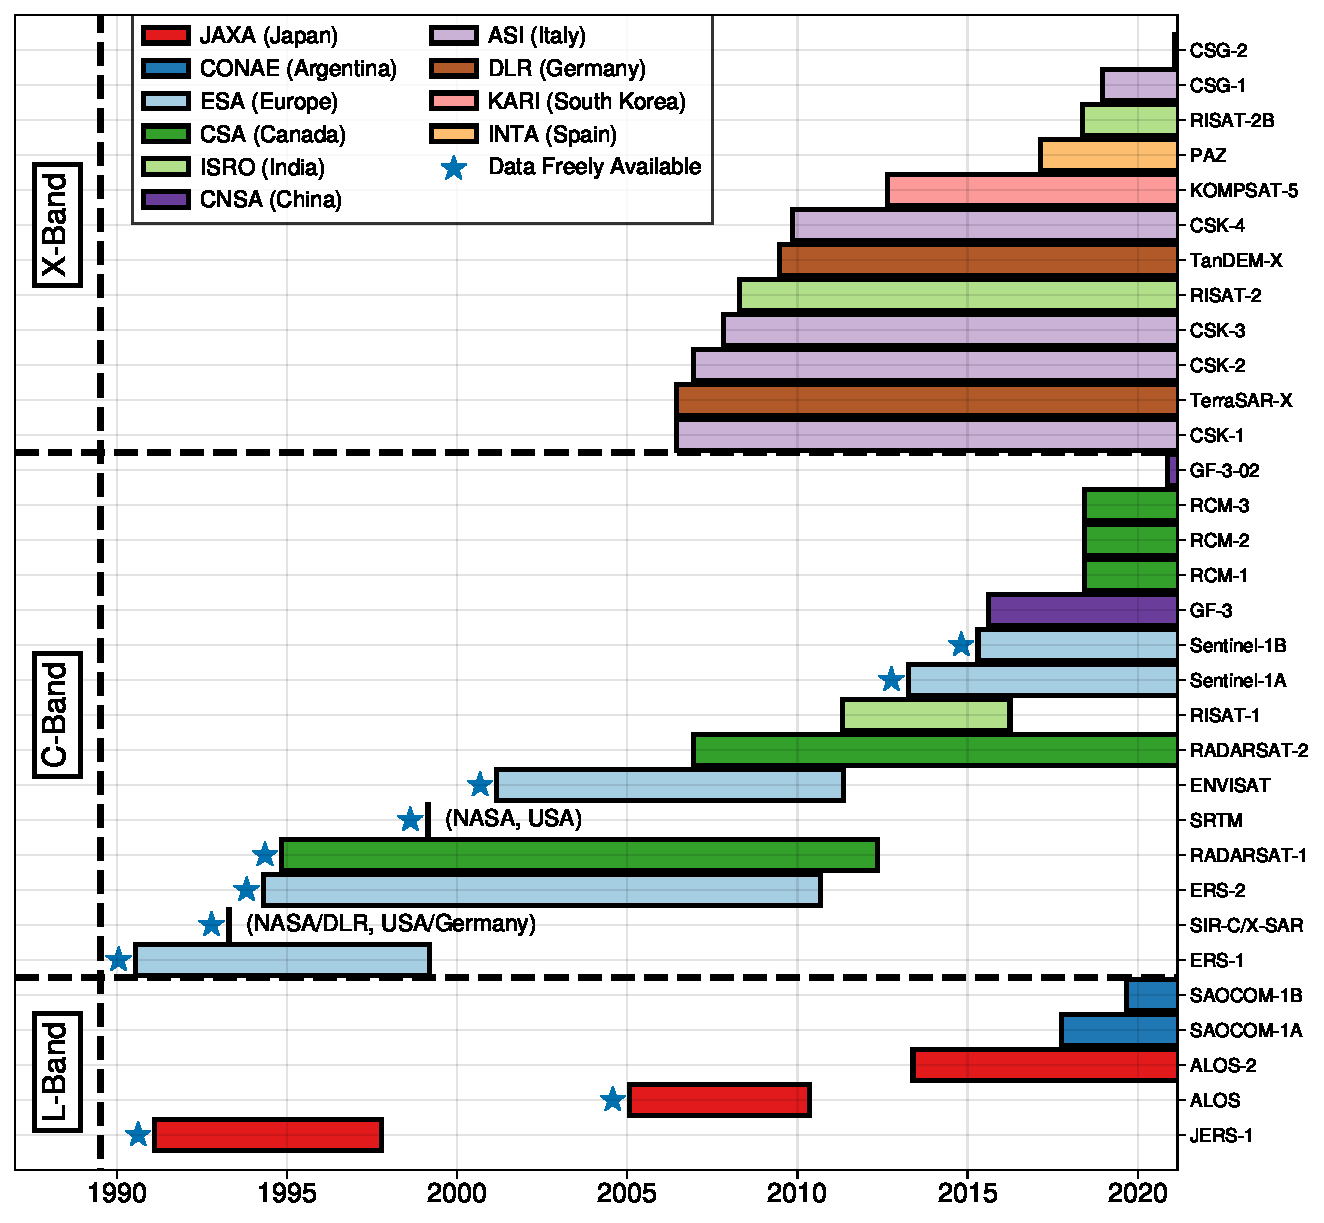
\includegraphics[width=1.\textwidth]{figures/chapter2-sar/sar-missions.pdf}
	\caption[Timeline of government SAR missions]{Timeline of government-sponsored SAR missions since 1990. Bar lengths indicate life span of mission. Bars which intersect the right edge indicate ongoing missions.
		Colors indicate the space agency operating the mission.
		Missions which provide data free of charge to the general public (as of May 2022) are marked with blue stars.
		Vertical sections of the timeline are divided by the radar frequency of the sensor, showing (from top to bottom) the X-band, C-band, and L-band missions.
		Note that SIR-C/X-SAR and SRTM were equipped with both C- and X-band sensors.	
%The acronyms for space agency operators or commercial owners are given in the legends. ASI, Agenzia Spaziale Italiana (Italian Space Agency); CNES, centre national d'etudes spatiales (France - National Centre for Space Studies); CONAE, Comisión Nacional de Actividades Espaciales (Argentina - National Space Activities Commission); CSA, Canadian Space Agency; DLR, Deutsches Zentrum fur Luft- und Raumfahrt (German Aerospace Centre); ESA, European Space Agency; INTA, Instituto Nacional de Técnica Aeroespacial (Spain - National Institute of Aerospace Technology); KARI, Korean Aerospace Research Institute; JAXA, Japan Aerospace Exploration Agency; NASA, National Aeronautics & Space Administration (USA).
}
	\label{fig:ch2-sar-missions}
\end{figure}


Figure \ref{fig:ch2-sar-missions} shows a timeline of SAR missions that have been launched by governments and space agencies since 1990. The missions are grouped vertically into the three most commonly used frequency bands for SAR sensors in earth-observing missions: L-band (wavelengths of $\sim$24 cm), C-band ($\sim$6 cm cm) and X-band ($\sim$3 cm).
During the 90s, the European Space Agency (ESA) launched two C-band SAR satellites: ERS-1 in 1991 and ERS-2 in 1995. The ERS-1 satellite provided the first practical demonstration of spaceborne InSAR's ability to capture surface deformation
when \cite{Massonnet1993DisplacementFieldLanders} mapped the surface deformation pattern caused by the 1992 Landers, California earthquake. The first L-band SAR satellite, JERS-1, was launched by NASDA\footnote{Although JERS-1 is labeled as a JAXA mission in Figure \ref{fig:ch2-sar-missions}, it was run by NASDA at the time. In 2003, NASDA merged with two other Japanese space agencies, ISAS and NAL, to form JAXA.} in 1992, and the Canadian Space Agency (CSA) launched their own C-band mission, RADARSAT-1, in 1995. In 2000, NASA flew the 11-day Shuttle Radar Topography Mission (SRTM) to generate the first high-resolution near-global topographical map of Earth \citep{Farr2007ShuttleRadarTopography}.

The most influential recent SAR mission within the science community has been Sentinel-1 \citep{Torres2012GmesSentinel1}. First launched in 2014, the Sentinel-1 satellites acquire data using the TOPSAR imaging mode which images very wide swaths ($\sim$240 km in the interferometry mode) \cite{Zan2006TopsarTerrainObservation}, allowing them revisit any point on Earth every 12 days.  Additionally, Sentinel is the first mission of its kind to provide free public data. This advanced SAR and InSAR from being an opportunistic study tool to  a operational technique to monitor nearly anywhere on Earth  \cite{Rosen2021ShiftingGround}. Sentinel-1 is currently the only active mission providing open SAR data; however, the future NISAR ISRO SAR mission (NISAR) will also provide free L-band SAR data with global coverage \citep{Rosen2015NasaIsroSar}.


\begin{figure}
	\centering
	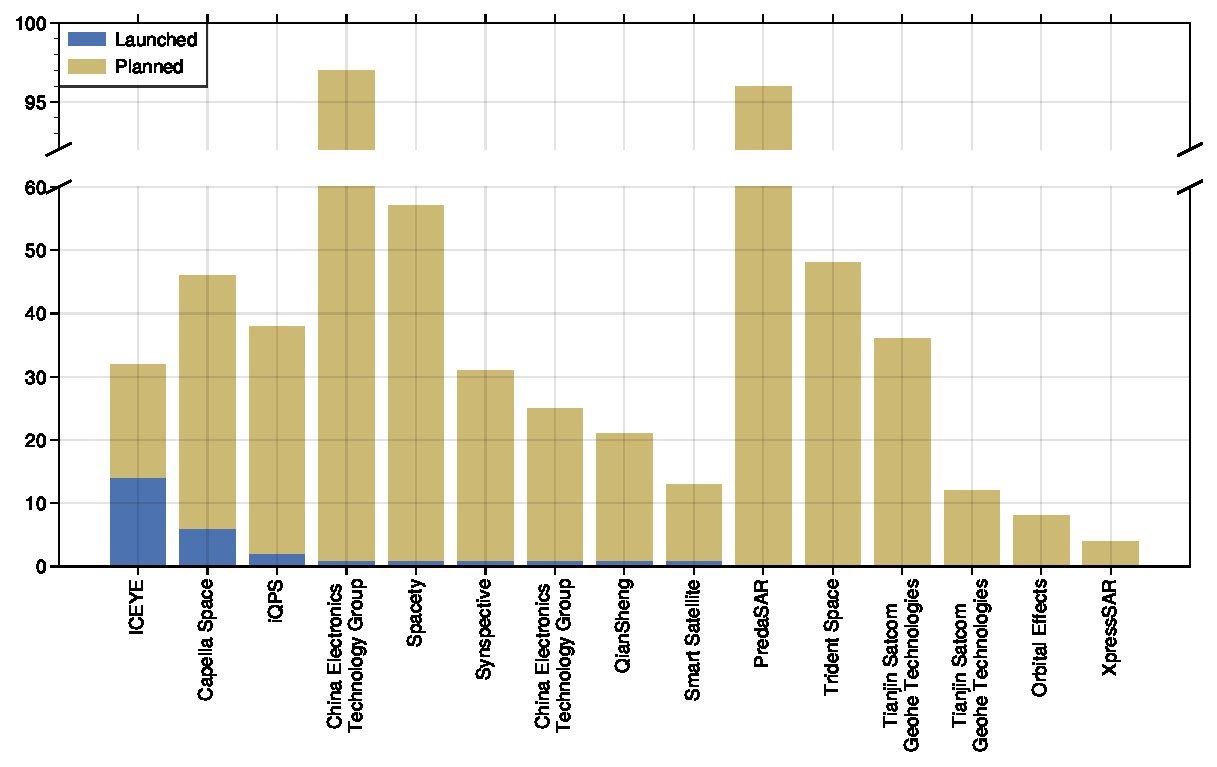
\includegraphics[width=1.0\textwidth]{figures/chapter2-sar/sar-private-constellations.pdf}
	\caption[Private sector SAR constellations]{SAR constellations run by private companies, showing the number of currently launched satellites (blue) stacked under the number of future planned launches (gold). Note the broken y-axis scale, as two companies 
		%	(China Electronics Technology Group and PredaSAR) 
		are planning constellations of 96 satellites.
	}
	\label{fig:ch2-sar-private-const}
\end{figure}



The first small SAR SmallSats (satellites weighing under 180 kg) have been launched by private companies over the past four years (Figure \ref{fig:ch2-sar-private-const}). Finland's ICEYE had its first succesful launch in January 2018, while Capella Space had their first launch 11 months later. Seven other companies have since launched at least 1 SAR satellite, and in the next five years, there are plans to launch over 500 additional SAR SmallSats \citep{Kulu2021SatelliteConstellations2021}. While many large SAR constellations expect sub-hourly revisit time for any given point on earth \citep{Stringham2019CapellaXband}, only the large government SAR missions, such as Sentinel-1, ALOS, and NISAR, explicitly plan for consistent global coverage in their mission objectives. However, the possibility of daily or hourly InSAR revisit times opens many new applications previously not possible with the 6-12 day revisit times of large SAR missions \citep{YagueMartinez2021TowardsFrequentFlood, Taylor2021RemoteSensingMountain, Kitajima2021PotentialSarSmall}.




\section{Synthetic Aperture Radar}
\label{sec:ch2-sar}


Synthetic aperture radar is an imaging technique that uses a radar mounted on a moving platform. A two-dimensional image is created by coherently processing the returned energy from transmitted pulses. While the images are often displayed in grayscale and may appear similar to optical images, they represent the electrical and geometrical properties of the objects in the scene \cite{Simons2007InterferometricSyntheticAperture}.
%To create a radar image, the energy scattered by points on the ground must be collected and focused in two dimensions.  The image represents the electrical and geometrical properties of the scene \cite{Simons2007InterferometricSyntheticAperture} 


The SAR imaging geometry is shown in Figure \ref{fig:ch2-sar-geometry}. A side-looking radar with look angle $\theta$ moves in the azimuth directory and repeatedly emits pulses at some interval (called the \emph{pulse repetition interval}, or PRI) which travel in the range direction.
%The illuminated portion of the ground has a swath width of $r \lambda / w$
%The width of the swath for stripmap operation is controlled by the antenna width, $w$, as $r \lambda / w$. Likewise, the size of the illuminated swath in the along track direction is $r \lambda / L$.
The line of sight (LOS) vector is defined as the unit vector pointing from the radar antenna to a point in the illuminated swath.
Each pulse illuminates a portion of the ground known as the radar footprint.


\begin{figure}
	\centering
		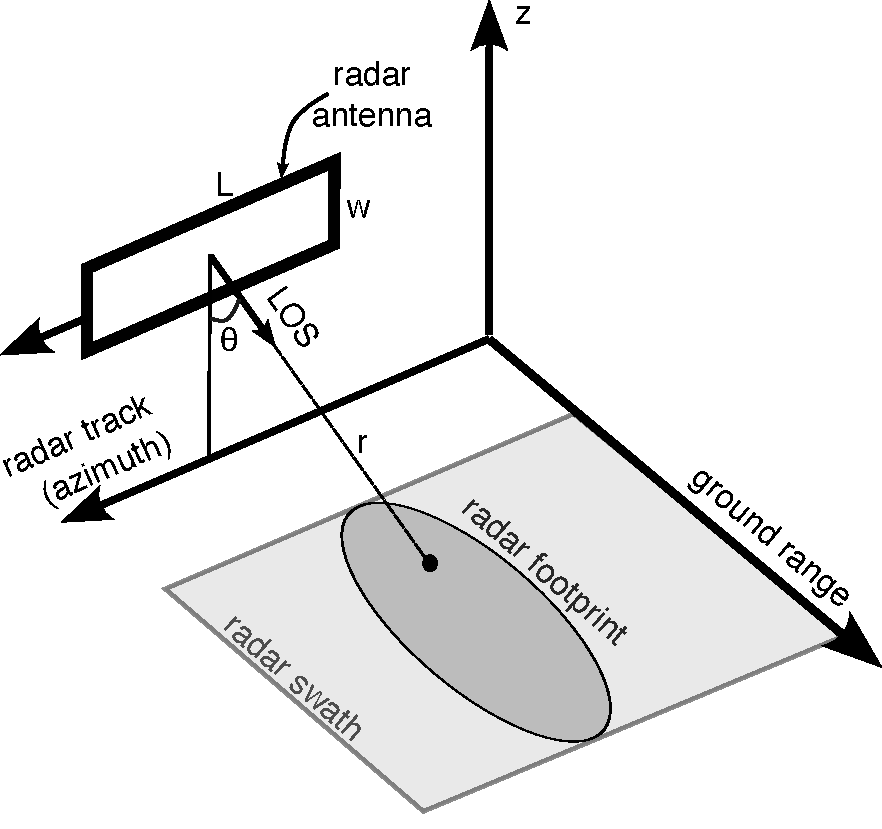
\includegraphics[width=0.99\linewidth]{figures/chapter2-sar/sar-geometry.pdf}
	\caption[Acquisition geometry of a SAR platform]{
	A platform moving in the azimuth/along-track direction contains a radar instrument with look angle $\theta$.    The slant range $r$ to the ground point is measured along the line-of-sight (LOS) direction from the antenna to the ground.
   	The radar antenna shown has length $L$ (in the azimuth direction) and width $w$.
   	As the radar sends out pulses, each one illuminates into an area on the ground called the beam ``footprint'' (oval shape). 
%   	As the platform moves and sends more pulses, they sweep out the radar swath (gray region).
	}
	\label{fig:ch2-sar-geometry}
\end{figure}

% Resolution: shorter pulse better resolution, but also lowers SNR. To get around tradeoff, send long with LFM chip to high snr and fine resolution in range direction


The signal-to-noise ratio (SNR) of the system depends on the total energy transmitted.  SNR can be increased by either sending a higher peak power (which is often limited by design constraints) or sending pulses with longer duration $\tau$. This choice creates a dilemma: in the absence further processing, sending pulses with a larger $\tau$ results in coarser range resolution $\delta_r$, where resolution is the ability to distinguish points illuminated by the same radar pulse. The illuminated size in range is $\delta_r = \frac{c \tau}{2}$, where $c \approx 3 \times 10^8$ is the speed of light. Thus, a pulse with $\tau = 30 $ microseconds would have a resolution of approximately 4.5 km. 

For this reason, SAR systems usually transmit pulsed waveforms called \emph{chirps} whose frequency $f$ increases or decreases over time. For example, in a linear frequency moduled (LFM) chirp, the frequency can be written as $ f(t) = k t$, where $k$ is the chirp slope (in Hz / s) and $-\tau / 2 < t < \tau/2$.
These special waveforms allow the receiver to correlate the returned echoes with a \emph{matched filter}, or a replica of the transmitted chirp. The improved range resolution depends on the frequency bandwidth of the chirp: $BW = f_{max} - f_{min}$.
For a given $BW$, the range resolution can be written as $\delta_r = \frac{c}{2 BW}$. 
%which means the resolution improves by a factor of $\tau \cdot BW$ (known as the \emph{time-bandwidth product}).


Figure \ref{fig:ch2-range-compress} demonstrates the effect of using a chirp waveform on range resolution. An example chirp with parameters matching the ERS-1 satellite (Figure \ref{fig:ch2-range-compress}a)
%The real part of an example chirp with parameters matching the ERS-1 satellite has an oscillation frequency which increases linearly over time (Figure \ref{fig:ch2-range-compress}a). 
has a duration of $\tau \approx 37.12 \mu s$ and chirp slope $k = 4 \times 10^{11} Hz / s$, resulting in frequency bandwidth $BW = k \tau$ $\approx$15.5 MHz (Figure \ref{fig:ch2-range-compress}b). By convolving the transmitted chirp with its complex conjugate, we get the impulse response of a point scatterer (Figure \ref{fig:ch2-range-compress}c). If a chirp with the same time duration had a smaller slope $k$ (Figure \ref{fig:ch2-range-compress}d), the bandwidth would shrink by the same proportion (Figure \ref{fig:ch2-range-compress}e), and the impulse response would also have worse resolution (Figure \ref{fig:ch2-range-compress}f).
Thus, we see that using chirped waveforms eliminates the original problem, as a pulse with larger bandwidth actually has a better resolution than a shorter pulse.


\begin{figure}
	\centering
%	\includegraphics[width=0.99\linewidth]{figures/chapter2-sar/range-compress.pdf}
	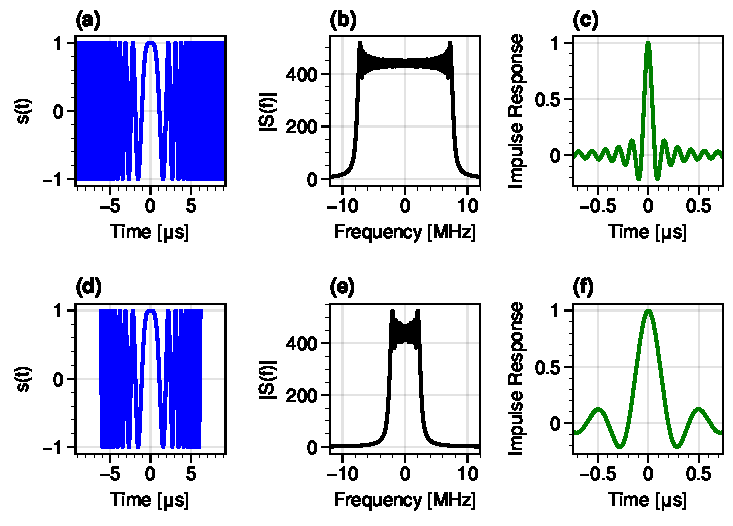
\includegraphics[width=0.99\linewidth]{figures/chapter2-sar/radar-chirp-bandwidth-ers.pdf}
%		\includegraphics[width=0.99\linewidth]{figures/chapter2-sar/radar-chirp-bandwidth-ers2.pdf}
	\caption[Range resolution from chirp compression]{
		(a) The real part of a linear frequency-modulated chirp with a duration of $\tau \approx 37.12 \mu s$ and a chirp slope $k = 4 \times 10^{11} Hz / s$.
		(b) The magnitude of the Fourier transform of the chirp is approximately a rectangle function, which shows the chirp bandwidth $BW = k \tau$ $\approx 15.5$ MHz.
		(c) Matched filtering of the returned echo from one point scatterer yields the impulse response, which shows the approximate 10 meters of range resolution (or $\sim$65 ns in time).
		(d) For a chirp with the same slope $k$ and 1/3 the duration $\tau$ the frequency bandwidth is also cut by 1/3 (e), the corresponding impulse response (f) and range resolution is 3 times worse.
	}
	\label{fig:ch2-range-compress}
\end{figure}


In the azimuth direction, the size of the radar footprint determines which ground points can be distinguished from the echo of one pulse;  this is known as the \emph{real aperture radar} (RAR) resolution. The footprint size can be written as $r \lambda / L$, which comes from the antenna's angular beam width $\lambda / L$ and the range $r$ to the target. The earliest imaging radar platforms were limited to this resolution in azimuth. For an airborne platform with a 1 meter antenna imaging at C-band, this would be a $\sim$600 meter resolution. Note that for some applications, such as military detection applications or wide-area ocean mapping \cite{Simons2007InterferometricSyntheticAperture}, this azimuth resolution is sufficient; however, the RAR resolution for spaceborne radars are on the order of 10s of kilometers, which is far too coarse for most applications.


%The advantages long wavelengths offer in terms of penetration come with compensating drawbacks. The resolution a sensor depends on the wavelength and on the size of its aperture—the mirror or lens in the case of a camera or a telescope, the antenna in a radar. If you lengthen the wavelength, you increase the size of the aperture you need in order to achieve a given resolution. To produce detailed images with radar requires a very large aperture indeed—far larger than anything a single spacecraft can offer.


\begin{figure}
	\label{fig:ch2-synth-aper}
	\centering
	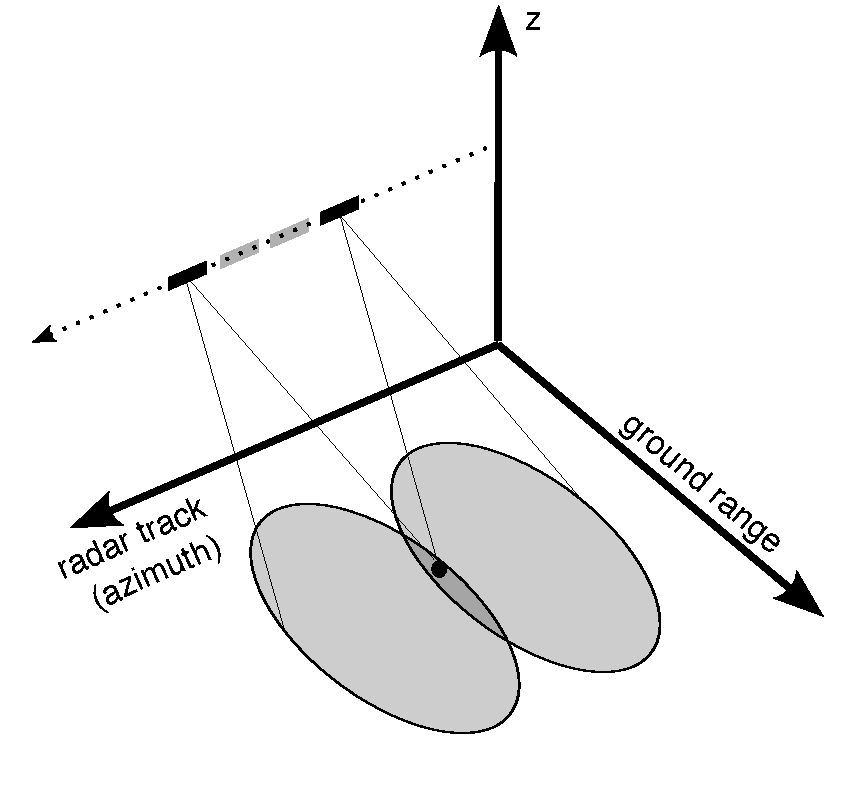
\includegraphics[width=0.75\linewidth]{figures/chapter2-sar/synth-aper2.pdf}
	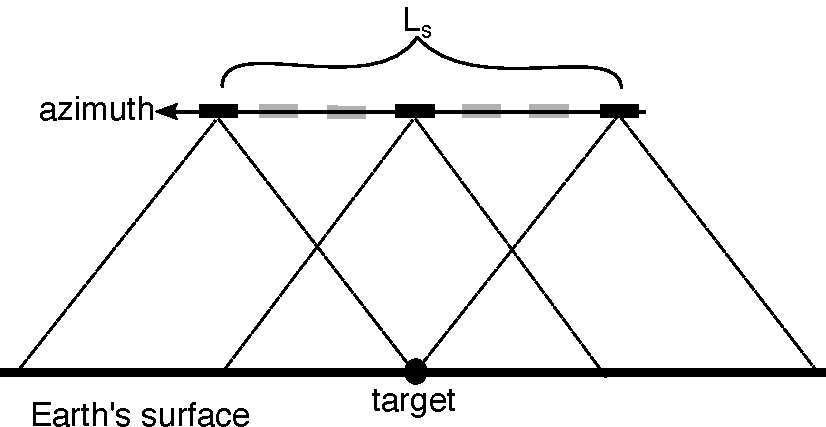
\includegraphics[width=0.95\linewidth]{figures/chapter2-sar/sar-synthetic-aperture.pdf}
	\caption[Formation of a synthetic aperture]{
		(Top) One point on the ground is illuminated by a series of pulses (only first and last pulses shown here) .
%		Pictured here are the footprints of the first and last pulses that illuminate the point. 
		(Bottom) Side view of a series of pulses illuminating a target. Coherently processing all pulses forms synthetic aperture of length $L_s$.
%		By coherently processing all pulses, we can form a synthetic aperture of length $L_s$.
	}
\end{figure}


The resolution in azimuth is greatly improved by creating a \emph{synthetic aperture}, which is a technique that processes the reflected echoes coherently (i.e. using both magnitude and phase) to focus the image (Figure \ref{fig:ch2-synth-aper}).
Coherent processing is possible by carefully tracking each target's phase history, $ \phi(t) $, which is related to the range to the target $r(t)$ 
\begin{equation}
\phi(t) = -\frac{4 \pi}{\lambda} r(t)  \label{eq:ch2-phase-range}
\end{equation}
There are multiple image formation algorithms which create this synthetic aperture and use the phase history. One of the first developed and most widely today used is the range-Doppler algorithm (RDA) \citep{Wu1976DigitalSystemProduce, Cumming1979DigitalProcessingSeasat}. 
RDA uses the apparent shift in Doppler frequency due to the platform motion to create a matched filter in azimuth, similar to the matched filter used for range compression \cite{Cumming2004DigitalProcessingSynthetic}.
%RDA is a frequency-domain algorithm, since it converts the phase history 
%Which converts the range-compressed data into the frequency domain. 
An alternative to RDA is time-domain backprojection \citep{Duersch2013BackprojectionSyntheticAperture}, which provides a more exact phase compensation at the cost of being more computationally expensive.
The backprojection algorithm collects the energy from every radar pulse containing a pixel and compensates for the range-dependent phase.
%To focus an image in azimuth using backprojection,
The complex-valued radar image $S$ (also known as a \emph{single-look complex} image, or SLC) at pixel location $ (x, y) $ can be formed by summing over all pulses and applying for a range-dependent term to cancel the propagation phase:
\begin{equation}
	S(x, y) = \sum_{k} s_k \left(t_k \right) e^{j \frac{4 \pi}{\lambda} r_k(x, y)}
\end{equation}
where $j = \sqrt{-1}$, $r_k(x, y)$ is the range distance from the radar sensor to the point $ (x, y) $ at the time of the $k$th pulse, $s_k(t_k)$ is the value of the $k$th range-compressed pulse at time $t_k = r_k(x, y) / c$, and $c$ is the speed of light \citep{Zebker2018InsarMissionLevel}.
%While computationally expansive, backprojection has become more common recently due to advances in computing hardware and 
If the radar imaging geometry is known precisely so that $r_k$ can be computed for all pulses, the coherent summation can be performed for each pixel to focus the SAR image.

For all image formation methods, the final achievable azimuth resolution $\delta_{az}$ is
%Processing all echoes coherently results in a fine resolution in the azimuth direction, which is equal to the resulting that would be attainable only by a real aperture of length $2 L_s$ \citep{Cumming2004DigitalProcessingSynthetic}.
%The phase of each return echo at a time $t$ is related to the range $r$ by $\phi(t) = -\frac{4 \pi}{\lambda} r(t)$.
\begin{equation}
	\delta_{az} = \frac{L}{2}
\end{equation}
where $L$ is the physical antenna length in the azimuth direction.
%Note the this final resolution is independent of wavelength, range or platform speed.
Normal spaceborne satellites have antennas on the order of 5-10 meters, resulting in a $\delta_{az} $ between 2.5-5 meters.
The intuition behind this surprising result is that, unlike with RAR, a smaller physical antenna size $L$ leads to a wider angular beam width $ \lambda / L$. This means that a given target is illuminated for a longer time, leading to a greater number of pulses to coherently process. Thus, the azimuth resolution will actually improve with a smaller antenna size.



\section{SAR Interferometry}

Interferometric synthetic aperture radar (InSAR) refers to a broad class of applications that exploit the phase difference between two SAR images to obtain extra information beyond the 2D locations of points \citep{Bamler1998SyntheticApertureRadar}. The most common applications are generating topography maps \citep{Graham1974SyntheticInterferometerRadar, Zebker1986TopographicMappingInterferometric} and mapping surface deformation \citep{Goldstein1987InterferometricRadarMeasurement, Gabriel1989MappingSmallElevation, Li1990StudiesMultibaselineSpaceborne, Massonnet1993DisplacementFieldLanders, Rosen2000SyntheticApertureRadar}. 
The InSAR measurement is made after precisely coregistering and resampling two SLC images $S_1$ and $S_2$ to the same coordinates. The phase measurement $I_{1,2}$ is formed by multiplying the first SLC $S_1$ by the complex conjugate of the second $S_2$: 
\begin{equation}
%	I_{1,2} = S_1 S_2^{*} = A_1 A_2 e^{j \left(\phi_1 - \phi_2 \right)}  \label{eq:insar-conj-mult}
I_{1,2} = S_1 S_2^{*} = A_1 A_2 e^{j \Delta \phi_{1,2}}  \label{eq:ch2-conj-mult}
\end{equation}
where $S_k = A_k e^{j \phi_k}$, $A_k$ is the amplitude of the $k$th image, and the phase $\phi_k = -\frac{4 \pi}{\lambda} r_k$. The image $I$ is called an \emph{interferogram},  and the quantity $\Delta \phi_{1,2} \triangleq  \phi_1 - \phi_2$ is the interferometric phase.

%TODO: 
TODO: summarize SRTM, and TANDEM X missions.
%
%maybe his topography stuff....
%- summarize SRTM, and TANDEM X mission
%- after into topo, can even mention missions to emphasize importance
%- for radar interferometry... mostly mention berardino chapter.


For topography mapping, two SAR antennas are separated by a distance in the across-track direction and each acquires a SAR image simultaneously\footnote{The acquisitions can also be at different times, under the assumption that no ground deformation has occurred.} (Figure \ref{fig:ch2-insar-geometry-topo}). The baseline causes the two radars to view the same point on the ground with a slight change in angle.
The difference in phase $\Delta \phi$ between $S_1$ and $S_2$ is related to the difference in the geometrical path length from each radar to the ground.
%: $\Delta \phi = \frac{-4 \pi}{\lambda}(r_1 - r_2)$. 
This means that $\Delta \phi$ changes based on whether the satellites are viewing flat ground (Figure \ref{fig:ch2-insar-geometry-topo}a) or topography (Figure \ref{fig:ch2-insar-geometry-topo}b). Thus, with precise knowledge of the viewing geometry, the height of the topography can be inferred from the interferometric phase for each point in the interferogram \citep{Simons2007InterferometricSyntheticAperture}. 
%Note that the phase difference can be thought of as a third measurement (in addition to the location in the azimuth and range directions) that allows a reconstruction of the 3D location of each image point \cite{Simons2007InterferometricSyntheticAperture}.


\begin{figure}
	\centering
	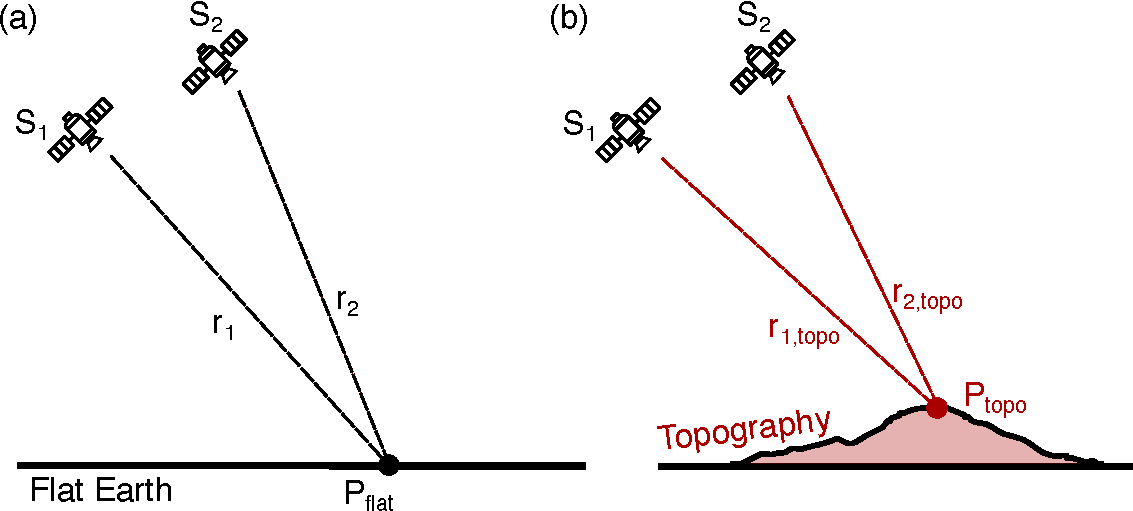
\includegraphics[width=0.99\linewidth]{figures/chapter2-sar/insar-geometry-topo.pdf}
	\caption[InSAR imaging geometry for topography mapping]{InSAR imaging geometry for topography mapping. Two SAR images, $S_1$ and $S_2$, are acquired with a slight spatial separation. The measured phase difference between $S_1$ and $S_2$ will change depending on whether we are viewing a point (a) on a flat Earth reference, or (b) at some topographic height.
%		 due to the change in look angles for each satellite.
%		(a)		 Two SAR images, $S_1$ and $S_2$, are acquired with a slight separation. The measured phase difference $\Delta \phi = \frac{4 \pi}{\lambda}(r_2 - r_1)$ results from the difference in geometric path length to the ground.
%		(b) $\Delta \phi$ changes when measuring topography due to the change in look angles for each satellite.
		 The this allows us to use the phase difference to infer the height of $P_{topo}$ above the reference Earth location $P_{flat}$.
	}
	\label{fig:ch2-insar-geometry-topo}
\end{figure}


In repeat-pass InSAR (sometimes called \emph{differential} InSAR, or DInSAR or DIfSAR)), a radar platform acquires two SAR images over an area acquired at different times, $t_1$ and $t_2$ (Figure \ref{fig:ch2-insar-geometry-defo}). Assuming that the topography is known and can be removed from the phase measurement, the remaining InSAR phase at each pixel measures the change in range along the radar LOS direction:
\begin{equation}
	\Delta \phi_{1,2} = \frac{4 \pi}{\lambda}(r_2 - r_1)   \label{eq:ch2-insar-phase-0noise}
\end{equation} 
%In the repeat pass setup, a small spatial baseline between the satellite at the two times is desired, while the topographic mapping application is more sensitive when the baseline is larger.
Since the measurement uses the phase of the propagated radar waves, it is only known modulo $2\pi$; the process of obtaining the full continuous phase is known as \emph{phase unwrapping}
\citep{Goldstein1988SatelliteRadarInterferometry, Chen2001TwoDimensionalPhase}. Note that even after phase unwrapping, the absolute number of $2\pi$ cycles from the radar to the ground is not known; thus, an unwrapped interferogram represents the surface deformation \emph{relative} to some point which is assumed to be zero.
Additionally, the description of the interferometric phase in Equation \eqref{eq:ch2-insar-phase-0noise} assumes no noise; in reality there are numerous noise sources which affect either the phase of an individual SAR acquisitions or the phase difference between pairs of images.



\begin{figure}
	\centering
	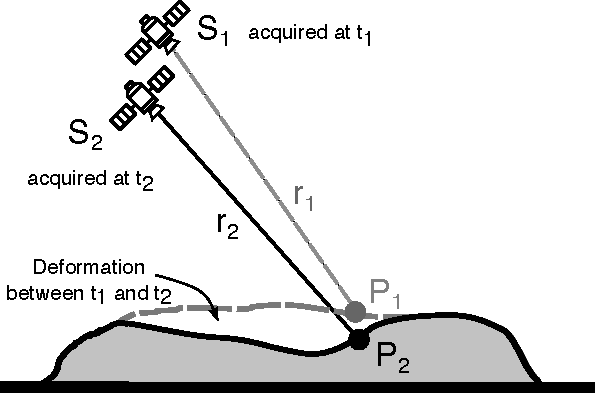
\includegraphics[width=0.9\linewidth]{figures/chapter2-sar/insar-geometry-defo.pdf}
%	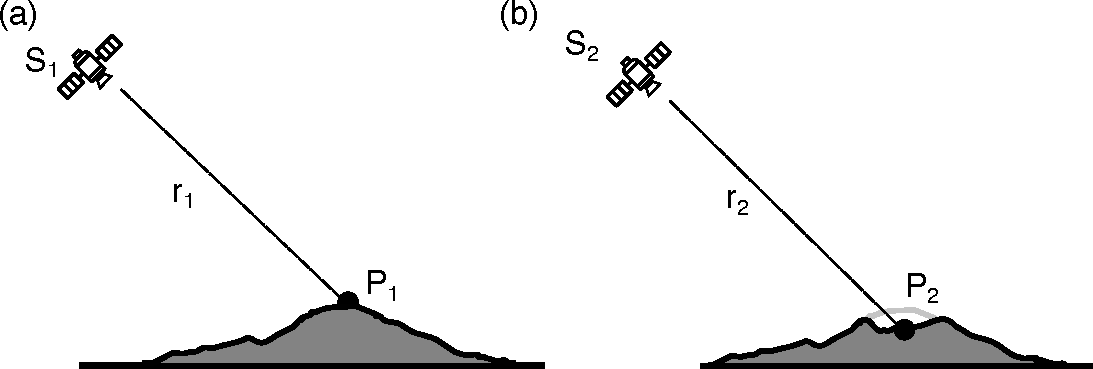
\includegraphics[width=0.99\linewidth]{figures/chapter2-sar/insar-geometry-defo-2col.pdf}
	\caption[InSAR imaging geometry for deformation mapping]{InSAR imaging geometry for deformation mapping.
		(a) Two SAR images, $S_1$ and $S_2$, are acquired at different times, before and after a ground deformation event. After removing the contribution from topography, the change in range between times $t_1$ and $t_2$ results in a measured phase change $\Delta \phi_{1,2} =  \frac{4 \pi}{\lambda}(r_2 - r_1)$.
	}
	\label{fig:ch2-insar-geometry-defo}
\end{figure}

\section{InSAR Noise Sources}
\label{sec:ch2-noise}
% decor
% atmo (further into iono/tropo, then tropo section)
%(maybe systematic for DEM/orbital,)
%thermal noise
%
After removing phase contributions from topography and satellite geometry, the phase at each pixel in an interferogram formed from SLCs $S_1$ and $S_2$ can be written as
%\citep{Zebker1992DecorrelationInterferometricRadar, Zebker1994AccuracyTopographicMaps, Zebker1997AtmosphericEffectsInterferometric, Hooper2006PersistentScatterRadar, Agram2010PersistentScattererInterferometry}
\begin{equation}
	\Delta \phi_{1, 2} = \frac{4 \pi}{\lambda} \left( \Delta d_{1,2} + \alpha_2 - \alpha_1 \right) + \Delta \phi_{iono} + \Delta \phi_{orb} + \Delta \phi_{dem} + \Delta \phi_{decor} + \Delta \phi_{unwrap} + \Delta \phi_{scat} + \Delta \phi_{n}  ,
	\label{eq:ch2-insar-noise-terms}
\end{equation}
where $ \lambda $ is the radar wavelength and $ \Delta d_{1,2} $ is the surface deformation between $S_1$ and $S_2$ along the radar LOS direction. 

The $\alpha_i$ terms represent the excess delay introduced by the neutral atmosphere on the $i$th day.
Tropospheric noise, $\Delta \phi_{tropo} \triangleq \alpha_2 - \alpha_1 $, arises from differences in pressure, temperature, or water vapor content between the two radar acquisitions \citep{Zebker1997AtmosphericEffectsInterferometric}.
%, which lead to changes in the index of refraction. 
Since tropospheric noise is the dominant noise for the West Texas study of Chapters \ref{CHAP:4-GRL}-\ref{CHAP:6-blob}, the noise is further detailed in Section \ref{sec:ch2-noise-tropo}.


Phase errors can also arise from variations in the index of refraction from due to ionospheric heterogeneities \citep{Gray2000InfluenceIonosphericElectron}. Since the ionosphere is a dispersive medium, the phase effects  $\Delta \phi_{iono}$ are dependent on radar frequency, with the effect at C-band being approximately 1/16 the effect at L-band \citep{Liang2019IonosphericCorrectionInsar}. Additionally, the dependence on frequency enables mitigation techniques which split the radar spectrum into sub-bands to calculate phase corrections \cite{Rosen2010MeasurementMitigationIonosphere}.
%with the index of refraction varying as $ \propto \frac{1}{f^2} $ \citep{Meyer2006PotentialLowFrequency}. 
%This means that 


The terms $ \Delta \phi_{orb} $ and $ \Delta \phi_{dem} $ represent systematic errors resulting from imprecise knowledge of the platform's orbital position or topographic height. Orbital errors usually appear as a planar phase ramp in stripmap acquisitions. Although these were common to see in ERS-1 or ENVISAT data, they rarely appear in Sentinel-1 data due to it's high precision orbit determination \citep{Fattahi2014InsarUncertaintyDue}. Errors in the DEM used to remove the topographic phase result in a spatial baseline-dependent phase error \citep{Fattahi2013DemErrorCorrection}. These errors often small in Sentinel-1 data due to the tight control of the repeat orbit tube, but can be significant in mountains or regions with sharp topography changes.

Decorrelation errors, $ \Delta \phi_{decor} $, arise from a loss of coherence of the phase between $S_1$ and $S_2$ due to changes in the surface dielectric properties or scattering characteristics \citep{Zebker1992DecorrelationInterferometricRadar, Michaelides2019AlgorithmEstimatingCorrecting, Ansari2018EfficientHighPrecision}. 
The correlation can be estimated from the complex coherence $\gamma $ of the interferogram \cite{Bamler1998SyntheticApertureRadar}
\begin{equation}
	\gamma = \frac{\left\langle S_1 S_2^{*} \right\rangle }{\sqrt{\left\langle S_1 S_1^{*} \right\rangle^2 \left\langle S_2 S_2^{*} \right\rangle^2}}
\end{equation}
where $ S_2^{*} $ is the complex conjugate of $ S_2 $ and $ \left\langle \cdot \right\rangle  $ denotes the statistical expectation operator. The expectation is defined as an ensemble average, but in practice it is estimated using some spatial window of pixels. 
The magnitude of this quantity $ \rho = |\gamma | $ is called the \emph{correlation} (or sometimes called the coherence), and varies from $ 0 $, indicating a complete loss of signal coherence, to $ 1 $, indicating perfectly correlated radar echoes.
%Decorrealtion 
When the correlation is very low, the phase unwrapping processing may fail and produce patches of pixels which have $2 \pi$ offsets from the correct value. These are known as phase unwrapping errors, $ \Delta \phi_{unwrap}  $. For study areas which regularly have strong decorrelation (e.g. agricultural areas), the technique known as persistent scatterer interferometry is used to overcome decorrelation by locating the phase-stable pixels which maintain coherence over long periods of time \citep{Ferretti2001PermanentScatterersSar, Agram2010PersistentScattererInterferometry, Hooper2006PersistentScatterRadar}.
%Note that because the angle of $\gamma$ is the interferometric phase, $\gamma$ may be considered the primary interferometric observable \citep{Michaelides2020QuantifyingPermafrostProcesses}.




The term $ \Delta \phi_{scat} $ represents phase introduced by changes to the surface and subsurface scattering properties. This term is separated from the random decorrelation noise since it has recently been shown that systematic, non-random effects can occur from changes to subsurface dielectric properties (e.g. from changes to soil moisture) \citep{Zan2014SarInterferometricModel, Zan2015PhaseInconsistenciesMultiple, Zwieback2015AssessmentSoilMoisture, Michaelides2020QuantifyingPermafrostProcesses}.
Although this term is noise for the application of deformation monitoring
\citep{Michaelides2019AlgorithmEstimatingCorrecting, Ansari2021StudySystematicBias}, other recent efforts have attempted to use this term to invert for changes to soil moisture \citep{Zwieback2017SoilMoistureEstimation, Zan2018VegetationSoilMoisture}. 
Finally, $ \Delta \phi_n $ represents other residual noise terms, including thermal noise from the radar antenna system, that are typically an order of magnitude smaller than the other errors listed.


Although these effects have been presented as noise sources for the application of deformation monitoring, they can be the signal of interest in other InSAR applications. For example, the presence of decorrelation indicates a change to the scattering surface properties and can be used for coherent change detection \citep{Simons2007InterferometricSyntheticAperture, Jung2016CoherentChangeDetection}, and the phase variations from the troposphere have been used for atmospheric mapping and meteorological purposes \citep{Hanssen1999HighResolutionWater, Liu2012SatelliteRadarInterferometry}.

% include orbital errors, phase decorrelation, unwrapping errors, DEM inaccuracies, ionospheric and tropospheric artifacts,
% and other residual noise terms that are typically an order of magnitude smaller than the error terms listed here.
%\begin{table}
%\begin{longtable}[]{@{}llcc@{}}
%	\toprule
%	Noise Symbol & Name & InSAR or SAR & asdf\tabularnewline
%	\midrule
%	\endhead
%	\phi_{orb} & & &\tabularnewline
%	\bottomrule
%\end{longtable}
%\end{table}


\subsection{Visual Example of Common Noise Sources}
\label{sec:ch2-noise-example}

In high signal to noise ratio (SNR) interferograms (e.g. for large magnitude earthquakes such as \cite{Massonnet1993DisplacementFieldLanders}), one can estimate the deformation magnitude by simply ``counting the fringes'' (i.e. visually estimating the number of $ 2 \pi $ cycles) and multiplying by $\lambda/2$. However, it is more common for an interferogram to contain many visual features corresponding to noise terms in Equation \eqref{eq:ch2-insar-noise-terms}. These noise sources can often be visually identified by InSAR experts, but they can add considerable difficulty for newer users without background knowledge of the study area.

\begin{figure}[!htbp]
	\centering
%	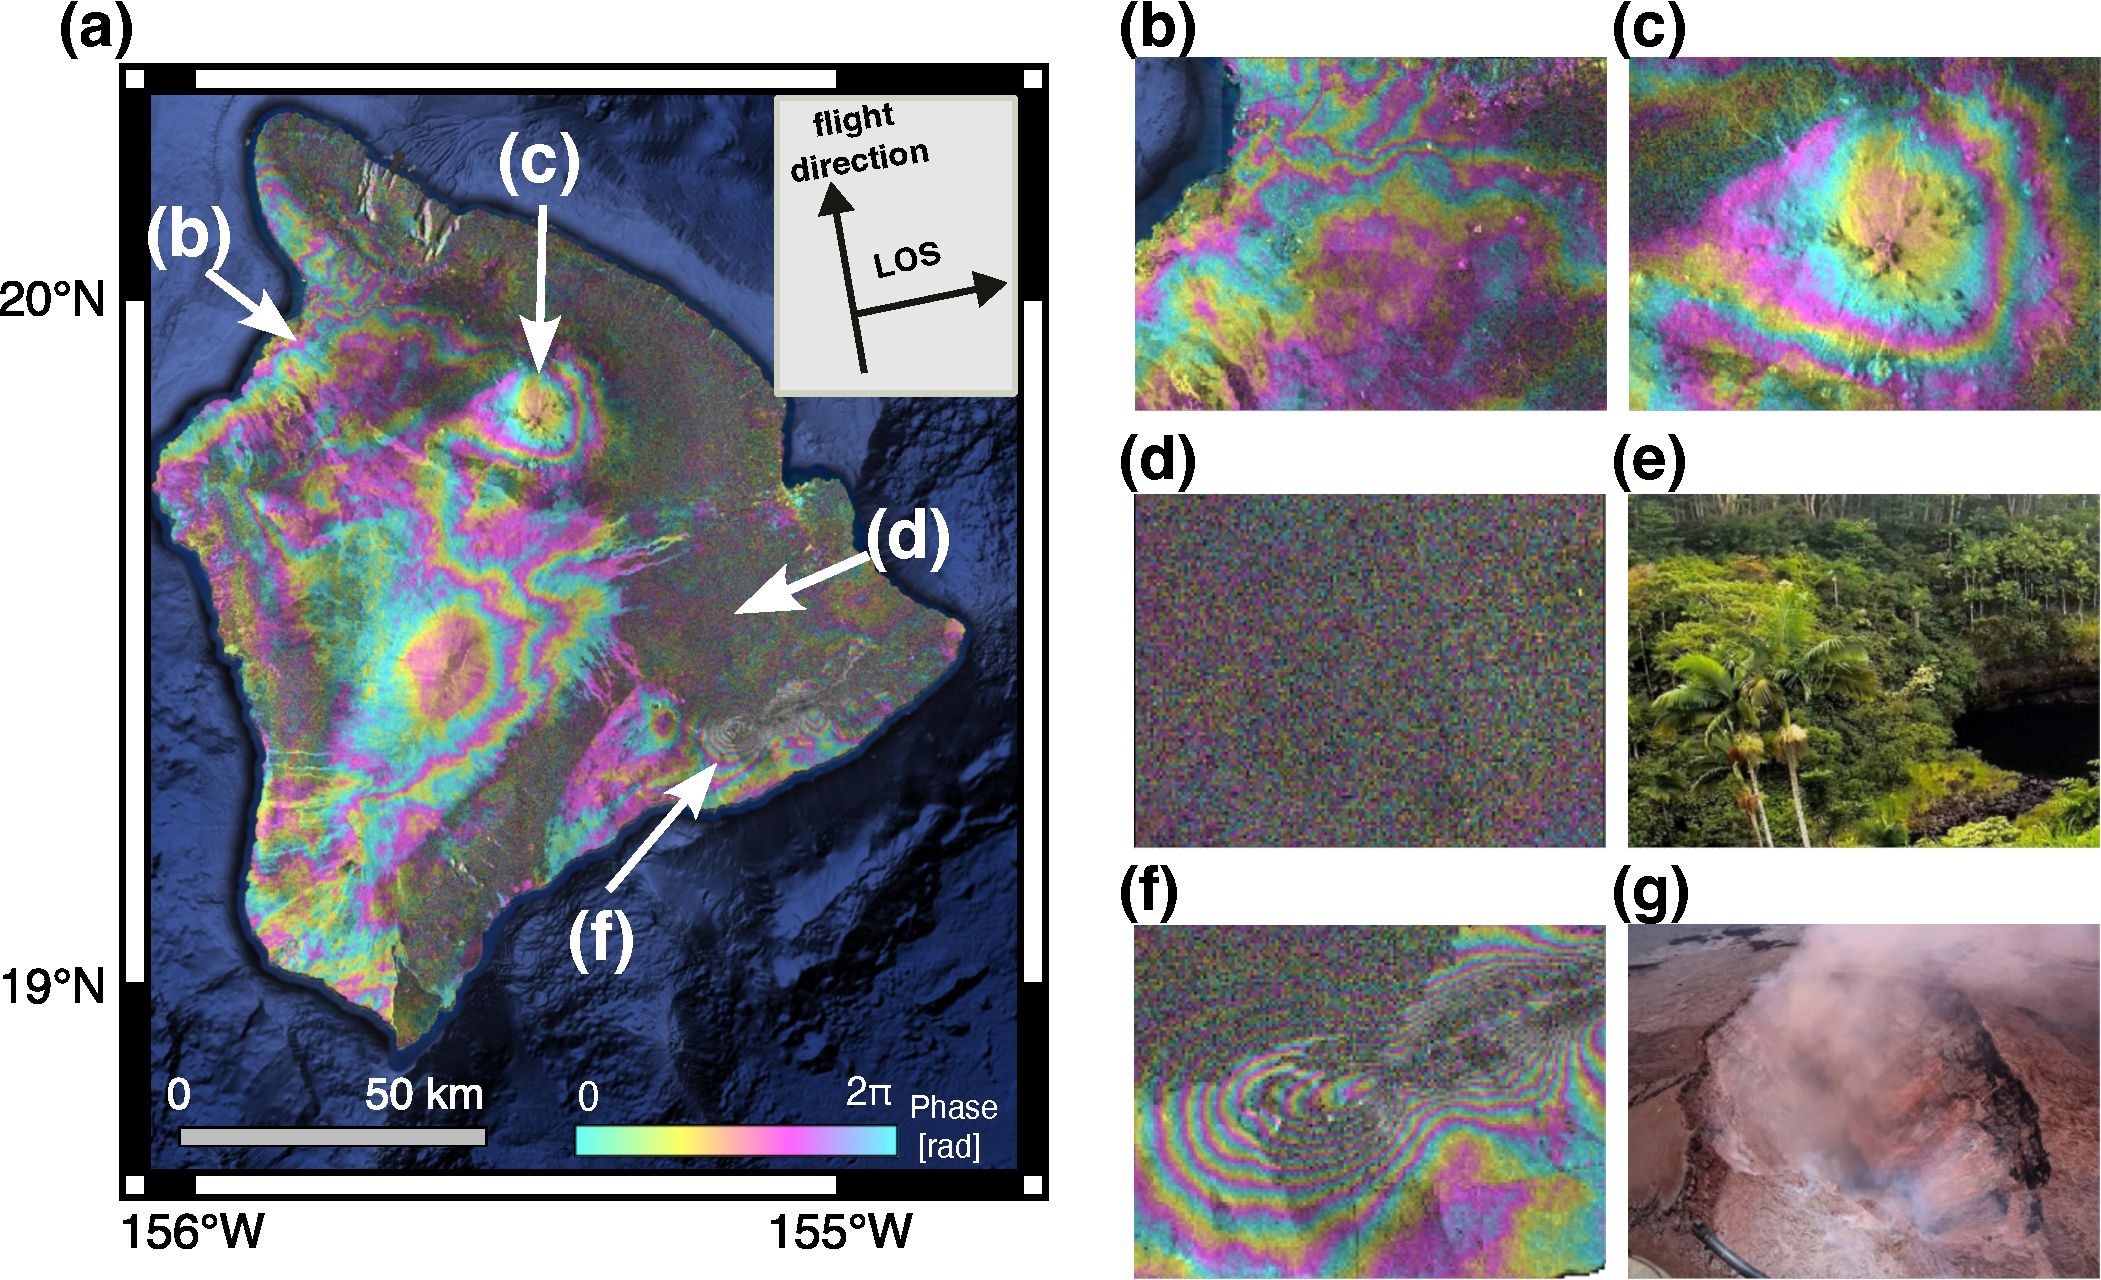
\includegraphics[width=1.0\textwidth]{figures/chapter2-sar/hawaii-example.pdf}
	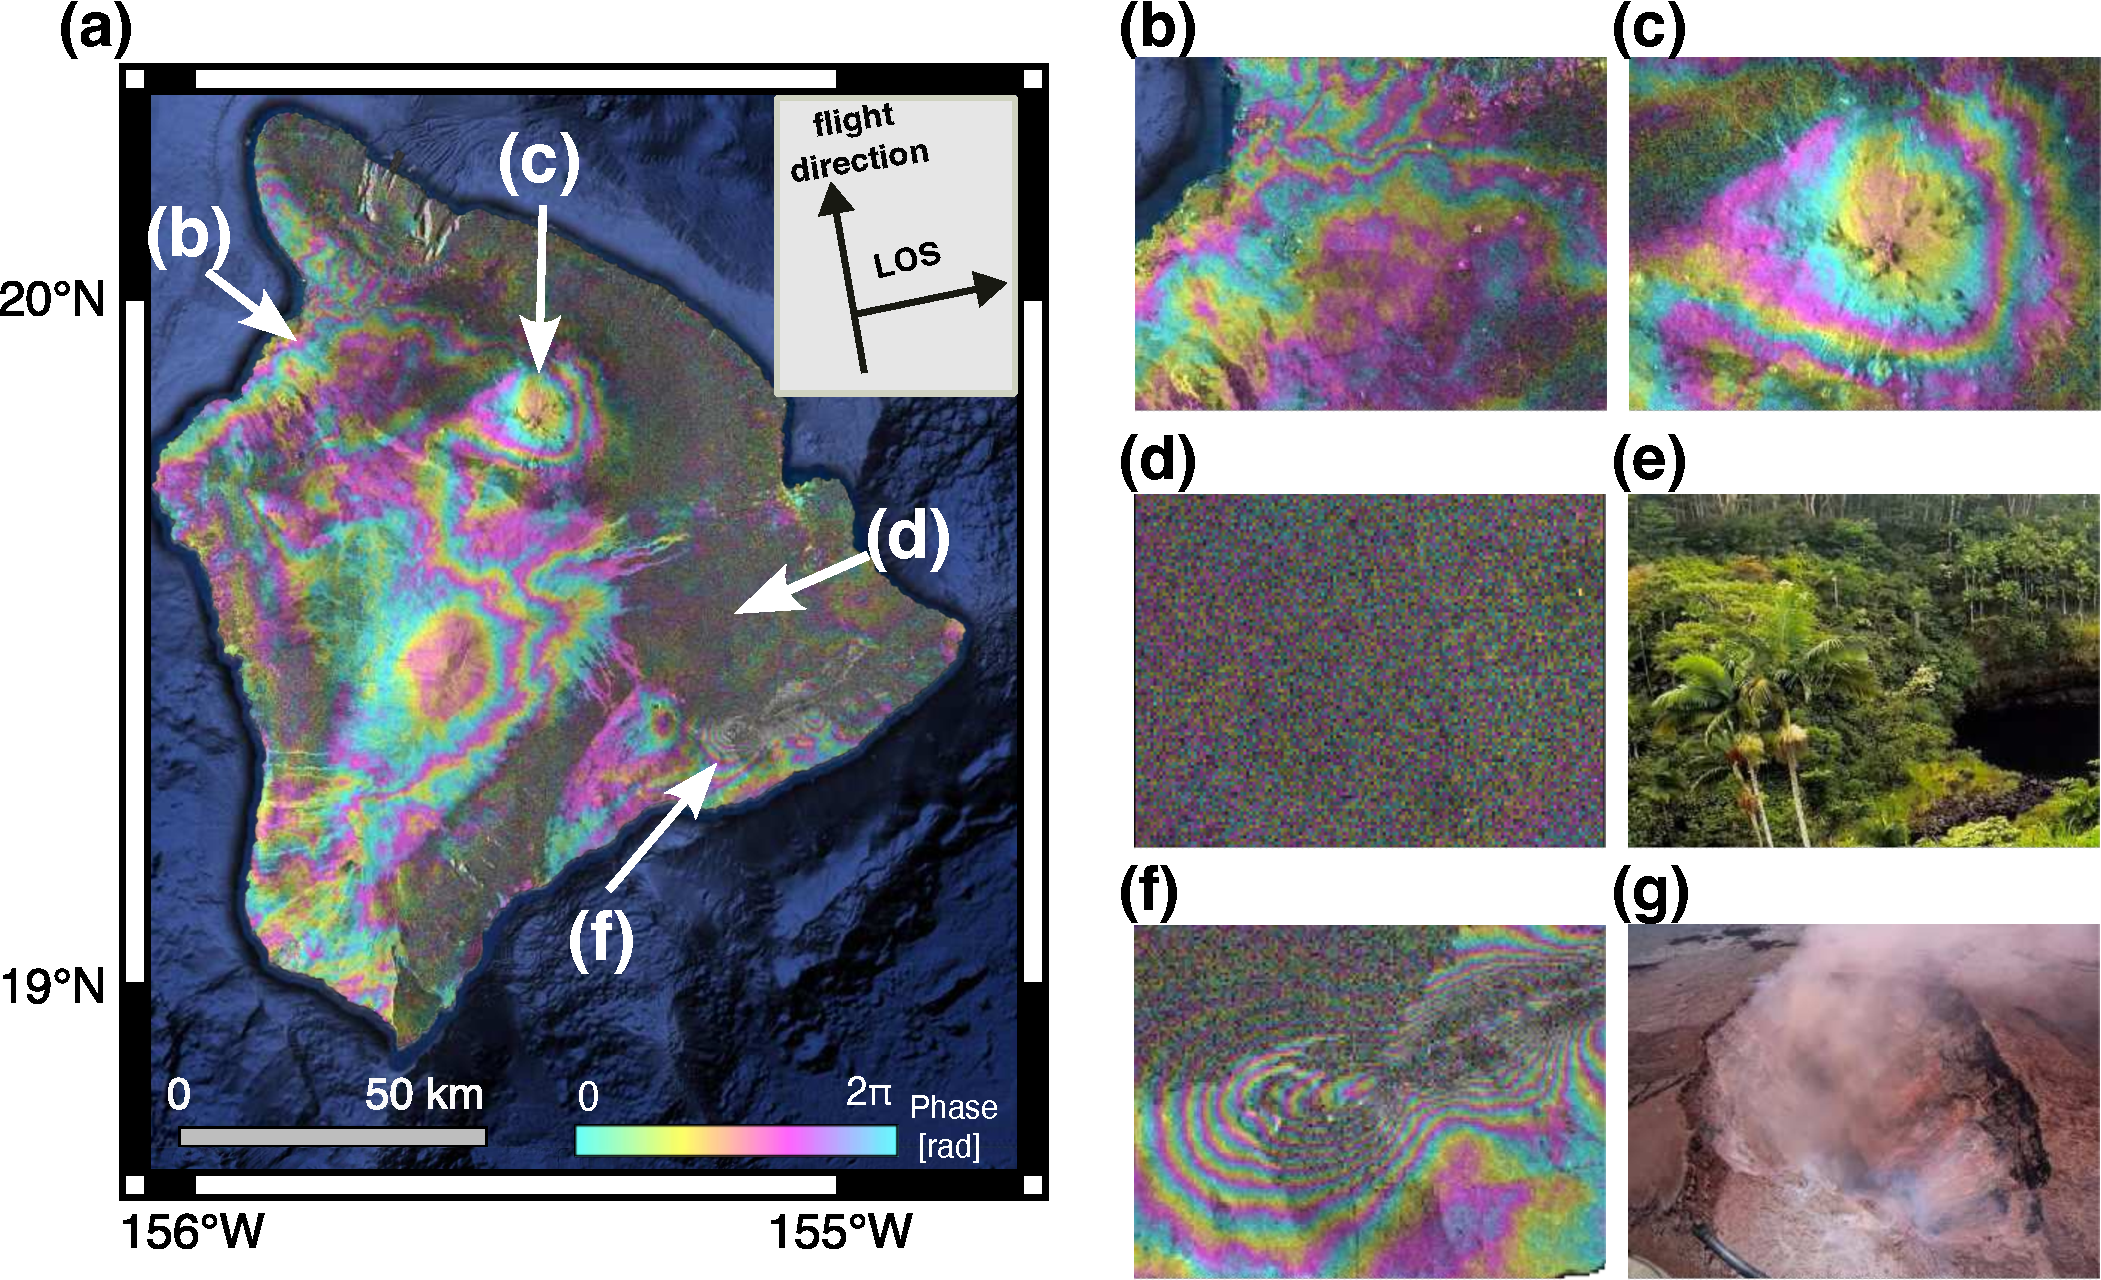
\includegraphics[width=1.0\textwidth]{figures/chapter2-sar/hawaii-example-small.pdf}
	\caption[Sentinel-1 interferogram over Hawaii showing common noise sources, along with 2018 eruption deformation]{
		(a) Sentinel-1 interferogram (ascending path 124) from April 20th, 2018 to May 2nd, 2018 over Hawaii, spanning the beginning of the 2018 K'\=ilauea eruption.
		Each colored phase cycle of $2\pi$ radians indicates a range change of 2.7 cm along the radar line-of-sight, which can be caused by real surface deformation or a noise source.
		(b) The dense fringes near the coast are caused by turbulent tropospheric noise (see Section \ref{sec:ch2-noise-tropo-mitigate}).
		(c) Stratified tropospheric noise on the peak of Mauna Kea, the tallest peak on Hawaii at 4,207 m, causes a concentric ring pattern. This pattern is also visible on Mauna Loa in the center of the island, where the phase is strongly correlated with topographic height. See Section \ref{sec:ch2-noise-tropo-mitigate} for further details.
		(d) An example of decorrelation noise caused by dense tropical rain forests (e) located on windward side of the island.
		(f) Real deformation of $ \sim 30-40 $cm around the Pu'u '\=O'\=o volcanic cone to the east of K'\=ilauea. In this case, the ground was subsiding down and to the southeast as magma flowed away from Pu'u '\=O'\=o.
		%		The signal of interest in this interferograms, the collapse of the Pu'u '\=O'\=o caldera
		(g) An aerial photo of Pu'u '\=O'\=o shows the caldera collapse on April, 30th, 2018 after magma migrated eastward underground (image source: HVO / USGS).
	}
	\label{fig:ch2-hawaii-example}
\end{figure}

To illustrate several common noise sources, Figure \ref{fig:ch2-hawaii-example} shows a Sentinel-1 interferogram of the Big Island of Hawaii from April 20th, 2018 to May 2nd, 2018. 
This time period spans the beginning of the 2018 Kilauea eruption during which a large subsidence event occurred from subsurface magma flow. However, the diversity in weather conditions, topography, and vegetation create many noise sources in most interferograms of Hawaii.
For example, the coastal region in Figure \ref{fig:ch2-hawaii-example}b contains dense fringes which could be mistaken as deformation, but in fact is due to turbulent tropospheric noise.
% (further explained in Section \ref{sec:ch2-noise-tropo-mitigate}).
The large elevation changes on Mauna Loa and Mauna Kea in the center of the island lead to stratified tropospheric noise,
%(see Section \ref{sec:ch2-noise-tropo-mitigate}) 
which creates a concentric ring pattern that is the same shape as a subsidence bowl (Figure \ref{fig:ch2-hawaii-example}c).
An example of decorrelation noise occurs on the windward side of the island (Figure \ref{fig:ch2-hawaii-example}d), which contains many dense tropical rain forests (Figure \ref{fig:ch2-hawaii-example}e). 

Finally, a real deformation feature of $ \sim 30-40 $ cm occurred near the Pu'u '\=O'\=o volcanic cone (Figure \ref{fig:ch2-hawaii-example}f).
In this case, the ground subsided down and to the southeast as magma flowed away from Pu'u '\=O'\=o (Figure \ref{fig:ch2-hawaii-example}g).
One can estimate the magnitude of deformation by counting the number of cycles in the interferogram in the zoomed-in region of Figure \ref{fig:ch2-hawaii-example}f and multiplying by 2.7 cm.
However, even this analysis can be difficult due to the high spatial frequency of the fringes.
For the Hawaiian case here, the deformation magnitude can be verified using nearby permanent GPS stations.

%These areas show heavy decorrelation at the Sentinel-1 C-band wavelength of 5.5 cm (Figure \ref{fig:ch2-hawaii-example}d). 

%
%Two days after the interferogram on May 4, a  M$_w$ 6.9 earthquake struck the south flank of the Lower East Rift Zone, just south of the zoom.


% at the Sentinel-1  
%brief fissure eruption occurred on the west flank of the Puʻu ʻŌʻō cone on April 30, 20181. Over the next few days, earthquakes migrated eastward into the LERZ and rift-normal displacements were recorded by GPS instruments, signaling large-scale injection of magma downrift of Puʻu ʻŌʻō. Magma reached the surface in Leilani Estates subdivision on May 3, marking the onset of the LERZ eruption (Fig. 1a)

%1. Table: noise, specific to ifg or SAR, max variance?, common?



\section{Tropospheric Noise}
\label{sec:ch2-noise-tropo}


% SEASONAL plots...??

The conversion between phase two-way distance from ground to satellite in Equation \eqref{eq:ch2-phase-range} assumes that the electromagnetic waves travel though a homogeneous medium with constant velocity. In reality, they travel through a spatially inhomogenous atmosphere with variable index of refraction $n$, where $n$ relates to the phase velocity $v$ and speed of light in a vacuum $c$ by $n = c/v$ \citep{Zebker1997AtmosphericEffectsInterferometric, Hanssen2001RadarInterferometryData, Liu2012SatelliteRadarInterferometry}.  Since $n$ is always real and slightly greater than $1$ for Earth's neutral atmosphere, it is more common to describe fluctuations using the \emph{refractivity} $N = 10^{6}(n - 1)$, which is the additional refractive index beyond unity.
Writing $N$ as $N(x,y,z)$ to emphasize the 3D variation, we can express the excess delay $D$ caused by the propagation through the atmosphere as
\begin{equation}
	D = 10^{-6} \int_{s} N(x, y, z) ds
\end{equation}
where $ds$ is the incremental slant length, and the integration runs along the radar line of sight. The excess delay adds an additional phase of $\phi = - \frac{4 \pi}{\lambda} D$ to a radar image acquired with the given atmospheric conditions.
%, and each interferogram contains a phase difference of two SLCs (i.e. the phase contains the difference from two atmospheric conditions).

The refractivity of the troposphere is commonly decomposed into a hydrostatic, wet, and liquid component \citep{Hanssen2001RadarInterferometryData, Bekaert2015StatisticalComparisonInsar}:
\begin{equation}
	N = \left(k_1 \frac{P}{T} \right)_{\text{hyd}} + \left( k_2^{'} \frac{e}{T} + k_3  \frac{e}{T^2}   \right)_{\text{wet}} + \left(k_4 W \right)_{\text{liquid}}
\end{equation}
where $ P $ is the total atmospheric pressure in hPa, $ T $ is the atmospheric temperature in Kelvin,  $ e $ is the partial pressure of water vapor in hPa, and W is the liquid water content of clouds in g/m$^3 $ 
The coefficients $ k_1, k_2^{'}, k_3 $ and $ k_4 $ are constants estimated from laboratory measurements, commonly taken to be $ k_1 = 77.6$ , $ k_2^{'} = 23.3 $, $ k_3= 3.75 \cdot 10^5 $, and $ k_4 = 1.45 $ from \cite{Smith1953ConstantsEquationAtmospheric} and \cite{Solheim1999PropagationDelaysInduced}.
%Although absolute delays decrease at lower altitudes as the signal travels through more of the atmosphere, an interferogram always measures a \emph{difference} of delays from two SAR acquisitions, and hence difference of refractivity. This means that although the hydrostatic delay is of the order of a few meters and the wet delay is $ \sim10$s of centimeters, phase artifacts in interferograms are more commonly caused by the spatial variations of the wet component of refractivity \citep{Zebker1997AtmosphericEffectsInterferometric, Hanssen2001RadarInterferometryData}. 
The hydrostatic delay is on the order of a few meters; however, it varies slowly laterally and it is often assumed to be vertically stratified (i.e. varying only with elevation) for small study areas (roughly $50 \times 50$ km or less) \citep{Doin2009CorrectionsStratifiedTropospheric}.
The wet component, caused by variations in water vapor content, is smaller in absolute terms ($ \sim10$s of centimeters) but has significant lateral variations at short length scales. The delay from the liquid component is often negligible (1-2 millimeters or less) but can be several centimeters in the presence of tall cumulonimbus clouds \citep{Liu2012SatelliteRadarInterferometry}.
For the purposes of InSAR analysis, noise from tropospheric delay is usually divided into a stratified component, which correlates with height \citep{Hanssen2001RadarInterferometryData, Doin2009CorrectionsStratifiedTropospheric}, and a turbulent component that is random at time scales longer than a day \citep{Emardson2003NeutralAtmosphericDelay, Onn2006ModelingWaterVapor}. 

%The hydrostatic delay is of the order of a few meters (Bevis et al., 1996) and the wet delay is usually not larger than 0.3 m (Elgered, 1982).
%The delay caused by droplets depends on the cloud type..
%ccording to Eq. (2.2.10) and the values of W listed in Tab. 2.1, significant delay up to 3 cm can be caused by the liquid water in vertical clouds, i.e., cumulonimbus (thunder clouds), which usually have a relatively limited horizontal size (< 10 km) and a large vertical extent and liquid water content. These clouds are typically generated by thermal convection or frontal lifting (Stull, 1995; Hanssen, 2001) \cite{Liu2012SatelliteRadarInterferometry}.


\subsection{Correction and Mitigation Strategies for Tropospheric Noise}
\label{sec:ch2-noise-tropo-mitigate}

%\subsection{Stratified Tropospheric Noise}
%\label{sec:ch2-noise-tropo-strat}
%\subsection{Turbulent Tropospheric Noise}
%\label{sec:ch2-noise-tropo-turb}

%Figure- GOES for storm cloud, and for weather front. Maybe there is where cite the reason why can't correct always.



Previous studies have made advances in correcting for the stratified component of tropospheric noise.  Several empirical approaches have been developed to fit linear or power-law relationships between the unwrapped phase and topography height of coherent pixels within interferograms \citep{Elliott2008InsarSlipRate, Lauknes2011InsarTroposphericStratification, Bekaert2015SpatiallyVariablePower, Zebker2021AccuracyModelFree, Murray2021ClusterBasedEmpirical}. Under the assumption that the deformation does not correlate with topography, these approaches can be effective and simple to implement. For example, Figure \ref{fig:ch2-hawaii-strat} shows the unwrapped interferograms from the area on top of Mauna Kea indicated in Figure \ref{fig:ch2-hawaii-example}c. Although the interferogram appears to show a bowl shape deformation (Figure \ref{fig:ch2-hawaii-strat}a), the phase is actually closely correlated with the topography (Figure \ref{fig:ch2-hawaii-strat}b-c). Fitting and removing a linear trend from the phase vs. elevation plot mitigates the stratified atmospheric noise in this case. However, these approaches can be less effective in regions with multiple weather patterns where the phase-elevation correlation can vary dramatically in space \citep{Murray2021ClusterBasedEmpirical}.

\begin{figure}
	\centering
	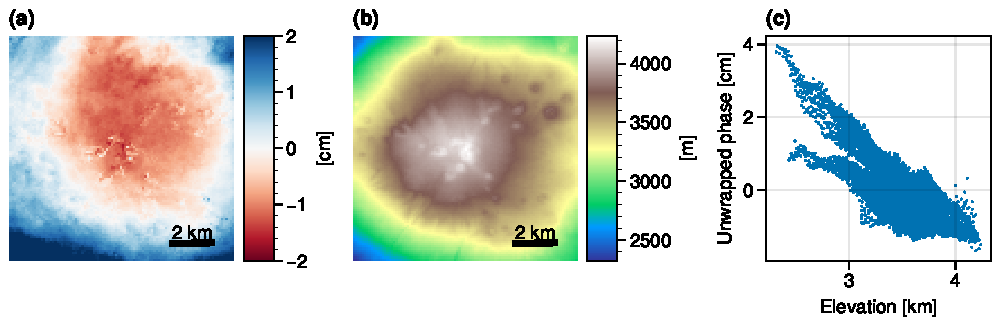
\includegraphics[width=1.0\textwidth]{figures/chapter2-sar/hawaii-strat-zoom.pdf}
	\caption[Stratified tropospheric noise over Hawaii]{
		(a) Unwrapped version of interferogram from Figure \ref{fig:ch2-hawaii-example}c, zoomed in to the top of Mauna Kea.
		(b) SRTM DEM heights for same area as (a)
		(c) Scatterplot of unwrapped phase (converted to centimeters) from panel (a) vs heights from panel (b) for all pixels.
	}
	\label{fig:ch2-hawaii-strat}
\end{figure}


Many efforts have advanced stratified noise corrections using auxiliary sources of data, including global atmospheric models (GAMs) \citep{Doin2009CorrectionsStratifiedTropospheric, Jolivet2011SystematicInsarTropospheric, Jolivet2014ImprovingInsarGeodesy, Cao2021AdvancedInsarTropospheric}, GPS zenith delay measurements \citep{Onn2006ModelingWaterVapor, Yu2017GenerationRealTime}, and external satellite measurements from sensors such as the Moderate Resolution Imaging Spectroradiometer (MODIS) \citep{Li2005InterferometricSyntheticAperture, Barnhart2013CharacterizingEstimatingNoise} or the Medium Resolution Imaging Spectrometer (MERIS)  \citep{Ding2008AtmosphericEffectsInsar}.
Several authors have attempted to create off-the-shelf correction services or toolboxes from these data sources. For example,	
\cite{Yu2018GenericAtmosphericCorrection} combined information from GAMs and available GPS zenith delay measurements to create the Generic Atmospheric Correction Online Service (GACOS) for estimating tropospheric noise in InSAR data. \cite{Maurer2021RaiderRaytracingAtmospheric} created a library for ray-tracing the LOS paths through GAM-predicted delays to create correction products.
While these correction methods show promise in certain study areas, the spatial and temporal resolution can be too low to correct for noise from severe weather or turbulent mixing of water vapor \citep{Murray2019TroposphericCorrectionsInsar}. Therefore, most methods for mitigating the turblent tropospheric noise rely on time series methods that exploit the uncorrelated temporal characteristics of the noise.
% on the atmospheric delay being uncorrelated for time scales longer than $\sim 6$ hours \cite{Emardson2003NeutralAtmosphericDelay}.


%
%\begin{figure}
%	\centering
%	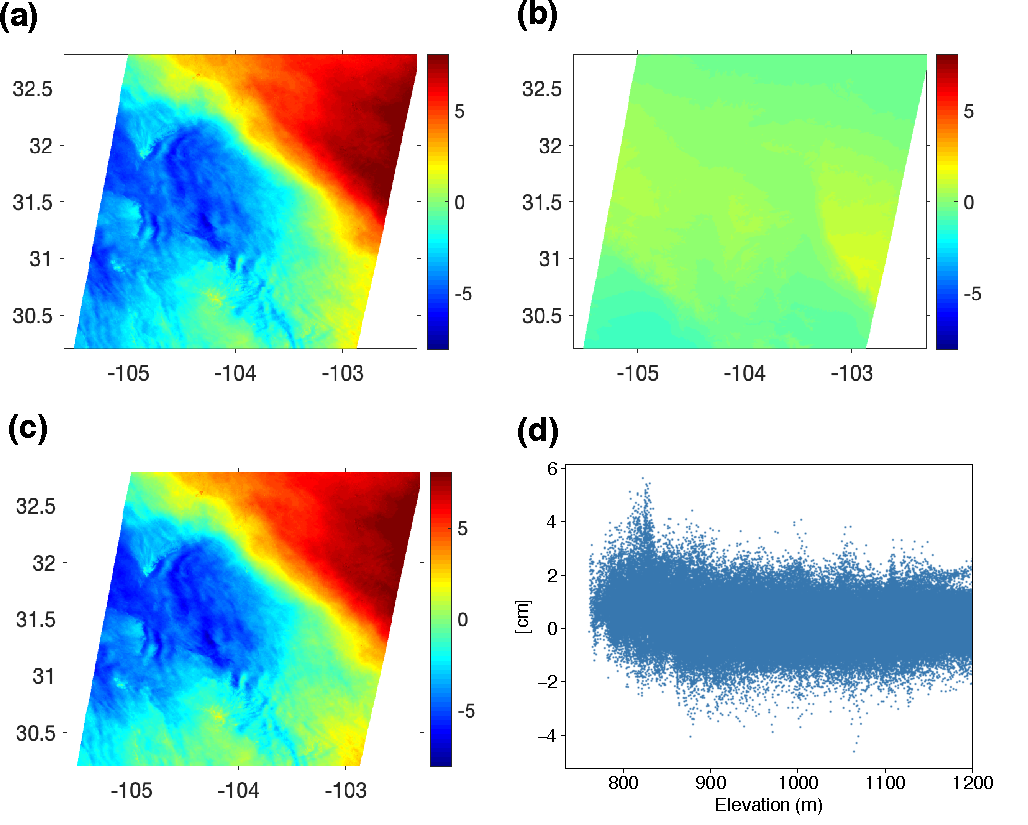
\includegraphics[width=\textwidth]{paper1-permian/figures/supplement/figureS4-gacos.pdf}		
%	\caption[GACOS tropospheric corrections]{(a) LOS measurements (in cm) of a descending interferogram (20150127-20150220) before the GACOS correction. (b) GACOS tropospheric correction (in cm) for the 20150127-20150220 interferogram \citep{Yu2018InterferometricSyntheticAperture}. (c) LOS measurements (in cm) of a descending interferogram (20150127 - 20150220) after the GACOS correction. (d) LOS measurements (in cm) of the 20150127-20150220 interferogram vs. the Digital Elevation Model (DEM).}
%	\label{fig:GACOS}
%\end{figure}


%In Chapters \ref{CHAP:4-GRL} and \ref{CHAP:5-robust-ts}, we 


\section{InSAR Time Series}
\label{sec:ch2-insar-ts}

%There are many techniques which fall under the umbrella of InSAR time series techniques, (sometimes called ``multi-temporal InSAR'' or MT-InSAR).
Since many noise sources cannot be distinguished from deformation in a single interferogram (e.g. Figure \ref{fig:ch2-hawaii-example}), it is common to analyze multiple interferograms 
%to quantify and mitigate InSAR noise sources.
using InSAR time series techniques (sometimes called ``multi-temporal InSAR'' or MT-InSAR), which extract information about the temporal evolution of surface deformation or other geophysical parameters of interest.  Most multi-temporal methods belong to one of the following categories: 1) stacking (averaging) \citep{Zebker1997AtmosphericEffectsInterferometric, Sandwell1998PhaseGradientApproach}, 2) small-baseline approaches \citep{Berardino2002NewAlgorithmSurface}, or 3) persistent-scatterer (PS) methods \citep{Ferretti2001PermanentScatterersSar, Hooper2006PersistentScatterRadar}. In the past decade, a fourth category of ``phase-linking'' approaches have been popularized by the SqueeSAR algorithm \citep{Ferretti2011NewAlgorithmProcessing}; these are based on optimizations or decompositions of the complex covariance matrix of SAR image stacks \citep{Guarnieri2008ExploitationTargetStatistics, Fornaro2015CaesarApproachBased, Ansari2018EfficientHighPrecision}. Methods (3) and (4) have shown success in extracting high-precision estimates of interferometric phase where decorrelation is the dominant noise source (e.g. in local, high-rate deformation, \citep{Tebaldini2010MethodsPerformancesMulti}); in the following section, we focus on (1) and (2).


For deformation signals which occur as a transient event 
%(which includes all processes quicker than one SAR acquisition interval) 
or with a constant rate, stacking consists of averaging multiple interferograms (possibly with different weights for each interferogram) which all contain the deformation signal \citep{Simons2007InterferometricSyntheticAperture, Zheng2019ImagingCascadiaSlow}. 
%Stacking approaches are the simplest conceptually and the earliest developed to mitigate tropospheric noise. 
For example, suppose an earthquake occurred at a known date, and we would like to estimate the coseismic displacement $\theta$ that occurred using a set of $M$ interferograms which all span the earthquake date. For each ground pixel, we can collect the phase difference measurements into a vector $\bm{\Delta \phi} \in \mathbb{R}^{M} $.
%\begin{equation}
%	\bm{\Delta \phi} = \left[ \Delta \phi_{1,2}, \Delta \phi_{1,3} , \ldots  \right]^T
%\end{equation}
To estimate the $\theta$, the simplest stacking solution is
\begin{equation}
	\theta = \frac{\lambda }{4 \pi} \frac{1}{M} \sum_i^M \bm{\Delta \phi}_i ,
	\label{eq:ch2-stacking-1}
\end{equation}
%consists of the $M$ phase differences for one ground pixel location, 
where $\bm{\Delta \phi}_i$ is $i$th element of the measurement vector, and the factor $  \frac{\lambda }{4 \pi} $ converts the phase from radians to centimeters.
For constant rate ground deformation, one approach based on \citep{Sandwell1998PhaseGradientApproach} to calculate the average LOS velocity $v_{avg}$ of each ground pixel is to compute
\begin{equation}
%	v_{avg} = \frac{\lambda }{4 \pi} \frac{\sum_{i \in G} d_i}{\sum_{i \in G} t_i}
	v_{avg} = \frac{\lambda }{4 \pi} \frac{\sum_i \bm{\Delta \phi}_i}{\sum_i \bm{\Delta t}_i }
	\label{eq:ch2-stacking-2}
\end{equation}
where $ \bm{\Delta t}_i $ is the temporal baseline of the $i$th interferogram (i.e. the time span $t_k - t_j$  for interferogram $ \Delta \phi_{j, k} $). %between SAR acquisitions at $t_j$ and $t_k$
%As noted by \cite{Simons2007InterferometricSyntheticAperture}, this method is equivalent to converting the interferogram measurements to rates and performing an averaging weighted by the respective time span.



% Yunjun thesis: the vector of interferometric phase residual that does not fulfill the zero phase closure of interferogram triplets. It includes the decorrelation noise, phase contribution due to the change of dielectric properties of ground scatterers such as soil moisture (De Zan et al., 2014; Morrison et al., 2011), processing inconsistency such as filtering, multilooking, coregistration and interpolation errors (Agram and Simons, 2015; Hanssen, 2001), and/or phase-unwrapping errors.

%An alternative objective function to solve equation (2.1) is minimizing the L2-norm of the residual of phase velocity of adjacent acquisitions (equation (16) in Berardino et al. (2002)). Optimizations with both objective functions give nearly identical solutions for a fully connected network



The Small Baseline Subset (SBAS) approach from \cite{Berardino2002NewAlgorithmSurface} formulates a linear estimation problem to solve for the phase at each SAR acquisition.
Suppose that the $M$ interferograms are formed from $N$ SAR acquisitions, where $ \frac{N}{2} \leq M \leq \frac{N(N - 1)}{2} $, and all interferograms have been unnwrapped and zero-referenced to a common location.
To solve for the LOS phase delay for each SAR acquisition $ \bm{\phi} = \left[\phi_0, \phi_1, \ldots, \phi_{N-1} \right]^T $, 
%we organize the system of equations as
we write the functional model of the linear system as
\begin{equation}
	\bm{A \phi} = \bm{\Delta \phi} + \bm{\epsilon} . \label{eq:ch2-sbas-A}
\end{equation}
where  $\bm{A}$ is the system design matrix, and $ \bm{\epsilon}  $ is the vector of interferogram-specific noise sources (e.g. $ \Delta \phi_{decor}, \Delta \phi_{unwrap}, \Delta \phi_{scat}, \Delta \phi_{n} $ from Equation \eqref{eq:ch2-insar-noise-terms}).
The matrix $\bm{A}$ is an incidence-like matrix where the row corresponding to measurement $ \Delta \phi_{j,k} \triangleq \phi_k - \phi_j $ has $1$ in the $k$th column and $-1$ in the $j$th column.
% (for all $j>0$).
Since interferograms are relative measurements, the first date's phase cannot be constrained and is conventionally taken to be $\phi_0 = 0$. Therefore, we omit the first column of the $ \bm{A} $ matrix containing $-1$ entries corresponding to $\phi_0$, leaving $N-1$ remaining terms in the unknown vector $ \bm{\phi} = \left[\phi_1, \ldots, \phi_{N-1} \right]^T $.
When $ \bm{A} $ is full column rank, the solution for $ \bm{\phi} $ can be obtained through least squares, $ \bm{\phi} = (\bm{A}^T \bm{A})^{-1}\bm{A}^T \bm{\Delta \phi}
 $, equivalent to minimizing the $L_2$ norm of the residual vector $\norm{\bm{A \phi} - \bm{\Delta \phi}}^2_2 $.

A common alternative to Equation \eqref{eq:ch2-sbas-A} is to solve for the phase velocity between each SAR acquisition $\bm{v} = [v_1, \ldots, v_{N-1}]^T$ where $ v_i = (\phi_i - \phi_{i-1})/(t_i - t_{i-1} ) $.
The linear system is now written as
\begin{equation}
	\bm{B v} = \bm{\Delta \phi} + \bm{\epsilon}, \label{eq:ch2-sbas-B}
\end{equation}
where the row of $\bm{B}$
corresponding to measurement $ \Delta \phi_{j,k} $ has $t_i - t_{i-1}$ in the $i$th column for $j < i \leq k$ and 0 elsewhere. 
After solving Equation \eqref{eq:ch2-sbas-B}, $ \bm{v} $ is integrated to obtain $ \bm{\phi} $.

The rationale behind solving for $\bm{v}$ is that for early SAR satellites, such as ERS-1 and ERS-2, the acquisitions are often grouped as subsets of images with small spatial baselines that are separated from other groups by large temporal or spatial baselines. 
When $\bm{\Delta \phi}$ contains an isolated subset of interferograms, $A$ is not full column rank and Equation \eqref{eq:ch2-sbas-A} is solved with a pseudo-inverse, $A^{\dagger}$, generated using the singular value decomposition (SVD) \citep{Strang2006LinearAlgebraIts}. The SVD approach for rank-deficient systems produces a minimum norm solution vector; the authors of \cite{Berardino2002NewAlgorithmSurface} found that minimizing the norm of the velocity vector $ \bm{v} $ produced more physically plausible deformation results than minimizing the norm of $ \bm{\phi} $. We note that for recent missions like Sentinel-1 with tightly controlled repeat orbits, it is often possible to create one connected network of interferograms, leading to equivalent results from the formulations of Equations \eqref{eq:ch2-sbas-A} and \eqref{eq:ch2-sbas-B}. However, Equation \eqref{eq:ch2-sbas-B} enables alternative regularization strategies for inversion, as shown in Section \ref{sec:ch4-method-compare}.
%and the system in Equation \eqref{eq:ch2-sbas-A} with full rank $ \bm{A} $ can be solved using least squares.



% ``Additionally, an atmospheric phase artifacts filtering operation is carried out on the computed space–time deformation measurements following the lines of the solution developed for the PS technique [16], [17]; in our case, the filtering operation takes benefit from the high spatial density of the imaged pixels''

%Note that this method relies on the assumption that the noise sources are uncorrelated (or weakly correlated) over time, as has been shown for tropospheric turbulence \citep{Emardson2003NeutralAtmosphericDelay}.


%% Appendix showing A/B? and maybe cumulative vector C? %%

%Note that \cite{Berardino2002NewAlgorithmSurface} solves each pixel independently, making parallel implementations straight forward.


%\citep{Schmidt2003TimeDependentLand} and \citep{Berardino2002NewAlgorithmSurface}.


%Since the turbulence noise cannot regularly be corrected, the noise statistics can be estimated.... \citep{Emardson2003NeutralAtmosphericDelay, Lohman2005SomeThoughtsUse}.
%Early efforts to correct or mitigate the turbulent atmospheric noise used a combination of high pass temporal filtering and low pass spatial filtering \citep{Ferretti2001PermanentScatterersSar, Berardino2002NewAlgorithmSurface}.
%- but as \citep{Liu2012SatelliteRadarInterferometry} notes, gaps in the acquistion, or strong non-Gaussianity from, e.g., severe thunderstorms, break the assumptions of equal variance among APS dates that these filters require.
%Several research efforts have attempted to produce estimates of the atmospheric phase delay for each SAR acquisition directly from a time series of interferograms. \citep{Liu2012SatelliteRadarInterferometry} formulated the problem as a linear system using a network of small baseline interferograms. Since the problem of estimating both surface deformation and atmospheric delay is an ill-posed problem given only differential InSAR measurements, the authors assumed zero or known deformation of the study region, and they constrained the estimated troposphere to have zero mean. In an attempt to denoise time series of surface deformation, \citep{Tymofyeyeva2015MitigationAtmosphericPhase} averaged sets of redundant interferograms containing a common reference date, with an assumption of linear or slowly-varying deformation, and subtracted the estimated troposphere. 

%An alternative approach to correcting for the tropospheric turbulence is to treat it as a stochastic noise source in time series analysis \citep{Simons2007InterferometricSyntheticAperture, Agram2015NoiseModelInsar} and estimate its covariance matrix either through auxiliary data sources \citep{Barnhart2013CharacterizingEstimatingNoise, Parker2015SystematicAssessmentAtmospheric} or directly from InSAR data \citep{Lohman2005SomeThoughtsUse}.



%\subsection{Uncertainty}
%\label{sec:ch2-eq-tropo}
%Several ways for uncertainty.
%
%jackknife (maybe look into the NSBAS/GIANT time series way they do it....). prob an underestimate, since this is *precision* of the estimator. often it's jsut precision of the noise+deformation phase. but we really want the defo phase.
%
%other is least squares propagation of covariance. difficult to calibrate without good atmo noise estimate, can underestimate/overestimate.
%
%one problem with daily time series: often uncertainty is a single number. but each day's atmo noise can vary by 10-20x.
%
%Even with temporal smoothing (example pic of that super storm cell), there can be many days with "blobs" of atmospheric noise which exceed real deformation.
%
%Chapter (2nd paper) will discus a third novel way using computer vision.
%
%
%Bootstrap:
%
%From "practictioners guide":
%A natural question for the practitioner is to ask  “ Why bootstrap in the linear regression case? Isn ’ t least - squares a well - established approach that  has  served  us  well  in  countless  applications? ”   The  answer  is  that  for  many  problems, least - squares regression has served us well and is always useful as  a first approach but is problematic when the residuals have heavy - tailed distributions or if even just a few outliers are present.
%
%IID assumption: doesn't hold for time series... still gives some estimate. maybe show example of how it overestimates, but that it's not bad because it's mostly accounting for tropo, and not for the phase UQ (cite Zwiebeck paper).


%Problems with pixelwise
%- Image of blob, with 8 mm cutoff, question which part you trust and not
%- Leads into feature-wise uq




\section{InSAR processing chain}
\label{sec:ch2-processing}
We developed software for an efficient and scalable InSAR processing chain to process geocoded SLC images and output cumulative surface deformation maps (Figure \ref{fig:ch2-processing}). An area of interest (AOI) is chosen in latitude and longitude coordinates, and all overlapping Sentinel-1 SLC products from a specified time frame are downloaded from the Alaska Satellite Facility (ASF) Distributed Active Archive Center (DAAC). The NASA Shuttle Radar Topography Mission (SRTM) \citep{Nasa2013NasaShuttleRadar} 30 meter DEM is downloaded for the AOI (stitching together tiles for regions larger than 1 x 1 degree) and upsampled.
The DEM, along with ESA's precise orbit files, are used by the Stanford processor \cite{Zheng2017PhaseCorrectionSingle, Zebker2017UserFriendlyInsar} to produce topography corrected, geocoded SLCs (GSLCs).
We note that working with GSLCs simplifies workflows for merging multiple Sentinel-1 frames over large areas \citep{Zheng2019ImagingCascadiaSlow}.
Interferograms are formed from the GSLCs through a pixel-wise cross multiplication (Equation \eqref{eq:ch2-conj-mult}), which are then unwrapped using the Statistical-cost, Network-flow Algorithm for Phase Unwrapping (SNAPHU) \citep{Chen2001TwoDimensionalPhase}. The unwrapped interferograms are referenced and (optionally) denoised by removing a planar or quadratic phase ramp. These are finally saved using the Hierarchical Data Format 5 (HDF5) data format, which allows user-defined metadata, data chunking, and compression.  HDF5 also simplifies and accelerates parallel implementations of pixel-wise SBAS algorithms (used in Chapter \ref{CHAP:4-GRL} and \ref{CHAP:5-robust-ts}).
%While equivalent interferograms can be produced by other software such as GMTSAR \citep{Sandwell2011OpenRadarInterferometry} or ISCE \citep{Rosen2012InsarScientificComputing}, 
% reduces the interferogram formation step to a simple cross multiplication, and they .
% as well as the ingesting future acquisitions  over the same AOI.



\begin{figure}
	\centering
	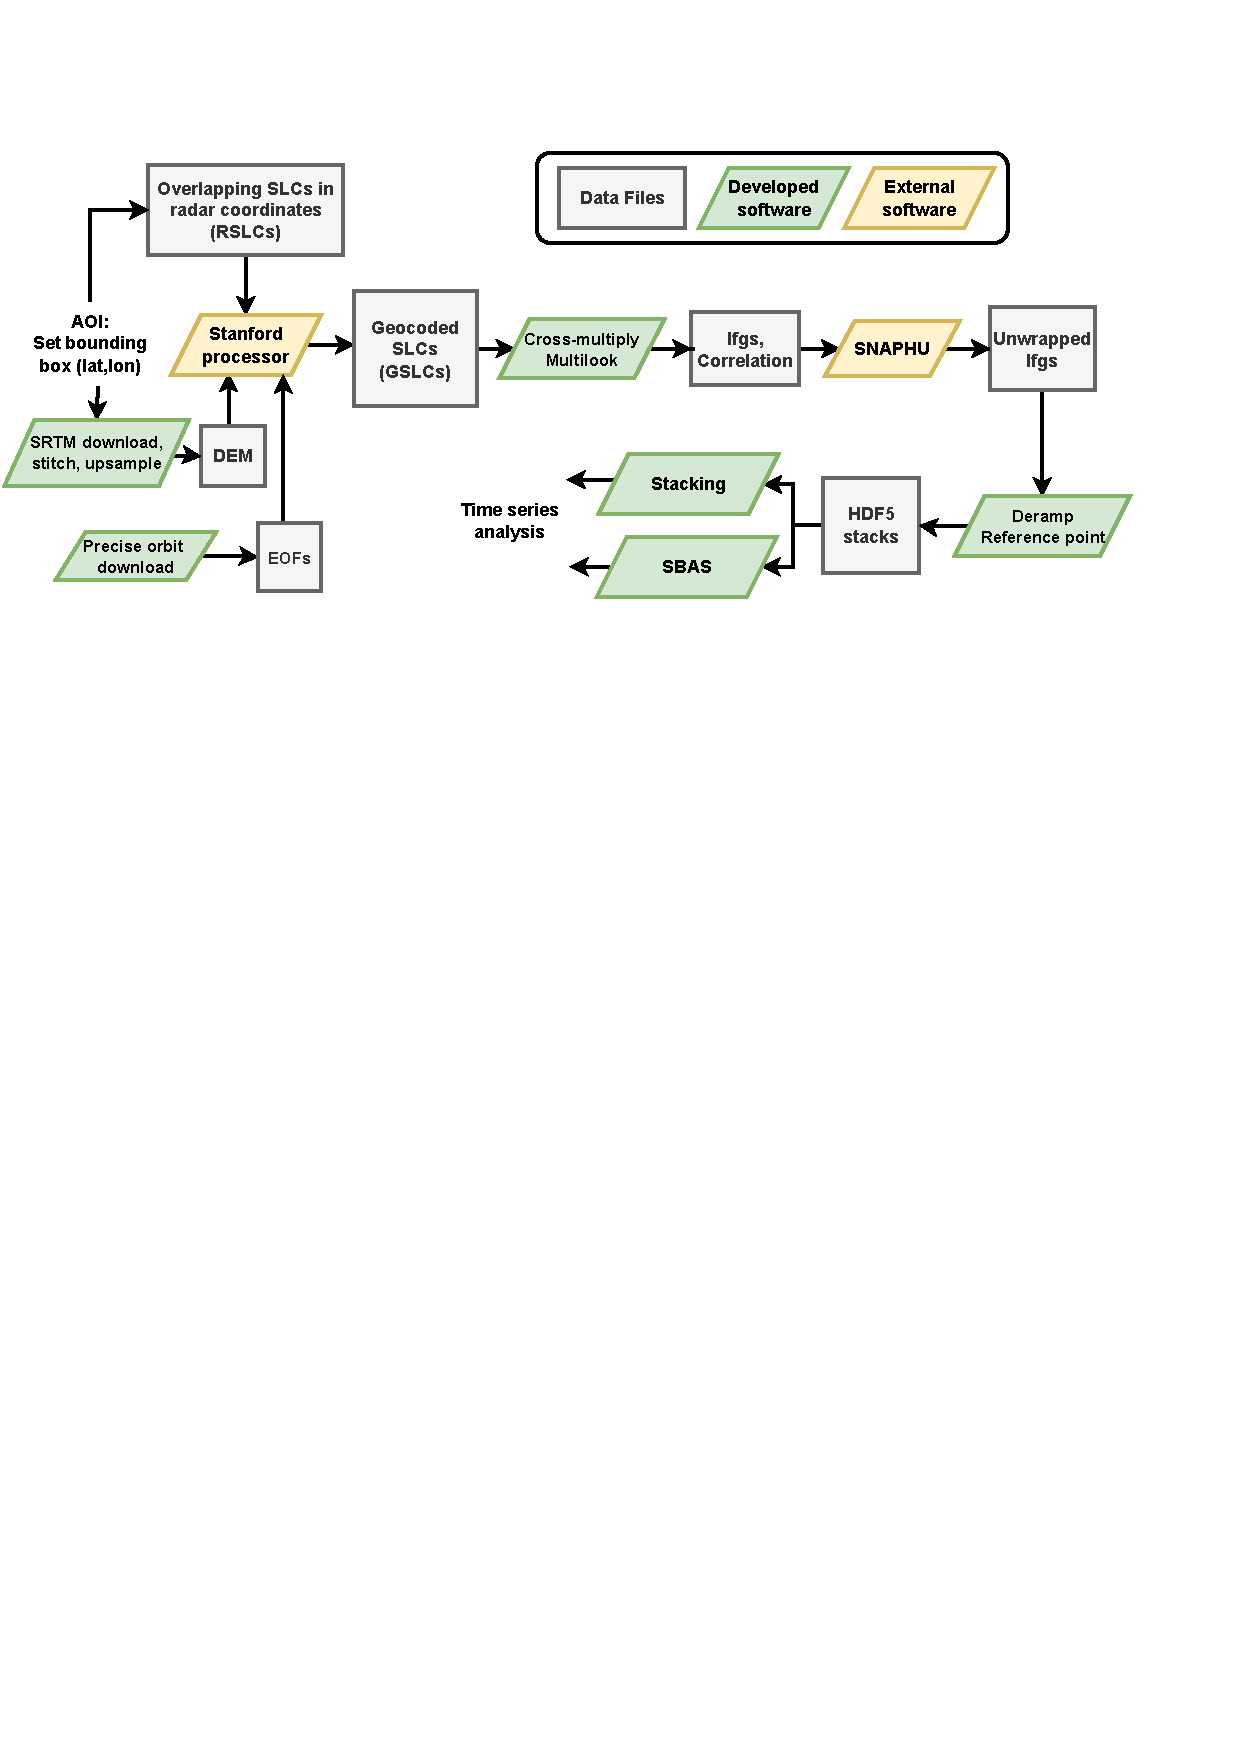
\includegraphics[width=\textwidth]{figures/chapter2-sar/processing-flow.pdf}
	\caption[Diagram of InSAR processing chain]{
	Processing chain used to create geocoded unwrapped of interferograms for stacking or SBAS time series analysis. Grey boxes indicate intermediate data products, yellow parallelograms indicate externally developed software packages, green parallelograms indicate software written for this thesis.
}
	\label{fig:ch2-processing}
\end{figure}


%- insatead of just TS formula, maybe mention the software... "geocoded SLCs". "write software into geocoded SLCs". "maybe one of the core group proc..."
%- somehow reflect that i can contribute to mintpy
%- one of key strengths... 'they can write fancy ts formula' they download software and run it... 
%- things i did aren't in mintpy... so could mention that the things will be developed for our radar interfeometry group
%- lot of people talk about algo method result... then you found they just ran code. "i ran this correction"
%- this was a reason she got hired. 
